

\documentclass[11pt, oneside]{article}   	% use "amsart" instead of "article" for AMSLaTeX format
\usepackage{geometry}                		% See geometry.pdf to learn the layout options. There are lots.
\geometry{letterpaper}                   		% ... or a4paper or a5paper or ... 
%\geometry{landscape}                		% Activate for rotated page geometry
\usepackage[parfill]{parskip}    		% Activate to begin paragraphs with an empty line rather than an indent
\usepackage{graphicx}				% Use pdf, png, jpg, or eps§ with pdflatex; use eps in DVI mode
								% TeX will automatically convert eps --> pdf in pdflatex		
\usepackage{amssymb}
\usepackage{amsmath} 
\usepackage{bm}
\usepackage{xcolor}
\usepackage{bbm}
\usepackage{bbold}
\usepackage[T1]{fontenc}
\usepackage{subfigure}
\usepackage[english]{babel}
\newtheorem{theorem}{Theorem}[subsection]
\newtheorem{corollary}{Corollary}[theorem]
\newtheorem{lemma}[theorem]{Lemma}
\newtheorem{mydef}{Definition}

%SetFonts

%SetFonts


\title{}
\author{}
\date{}							% Activate to display a given date or no date

\begin{document}
\maketitle 
\section{General Notations}

\begin{itemize}

	\item {$N$: Number of users}
	
	\item {$n$: Number of items,    $
	n = \left \{
	\begin{aligned}
	&2m-1, && \text{if n is odd} \\
	&2m, && \text{otherwise}
	\end{aligned} \right.
	$}
	
	\item{$\mathcal{P}_n$: the space of permutation of $n$ items}
	\item {$\bm{R}^1,...,\bm{R}^N$: full rankings given by the users}
	
	
	\item {$\bm{R}^j \in \mathcal{P}_n$= \{$R^j_1,...,R^j_n$\} $\sim$ Mallows($\bm{\rho}^0, \alpha^0$), defined as 
	$P(\bm{R}^j|\alpha^0, \bm{\rho}^0) = \frac{\text{exp}\{-\frac{\alpha^0}{n}d(\bm{R}^j, \bm{\rho}^0)\}}{\sum\limits_{\bm{r}\in \mathcal{P}_n}\text{exp}\{-\frac{\alpha^0}{n}d(\bm{R}^j, \bm{\rho}^0)\}}$}
	
	
	\item {$P(\bm{\rho}|\bm{R}^1,...,\bm{R}^N,\alpha^o)$: Mallows posterior}
	
	
	\item{\{$i_1, ..., i_n$\}: a ranking of $n$ items that determines the sequence following which the items are to be sampled. i.e. $i_j = k$ indicates that item $j$ is the k-th item is to be sampled}
	
	\item{ \{$o_1, ..., o_n$\}: an ordering of $n$ items that corresponds to \{$i_1, ..., i_n$\} s.t. $i_{o_k} = k$ }. $\{o_1, ...,o_n\}$ and \{$i_1, ..., i_n$\} have a one-to-one relationship
	
	%pseudo components 
	\item {$Q(\tilde{\bm{\rho}}|\cdot)$=$\sum\limits_{\{i_1, ..., i_n \}\in \mathcal{P}_n }q(\tilde{\bm{\rho}}|i_1, ..., i_n, \alpha_0, \bm{R}^1, ...,\bm{R}^N) \cdot g(i_1, ..., i_n| \dots)$ : pseudolikelihood that approximates the Mallows posterior}
	
	\item {$q(\tilde{\bm{\rho}}|i_1, ..., i_n, \alpha^0, \bm{R}^1, ..., \bm{R}^N)  = q(\tilde{\bm{\rho}}|o_1, ..., o_n, \alpha^0, \bm{R}^1, ..., \bm{R}^N)  \\
		=q(\tilde{\rho}_{o_1}|\alpha^0,o_1, R^1_{o_1},...,R^N_{o_1}) \cdot
		q(\tilde{\rho}_{o_2}|\alpha^0,o_2,\tilde{\rho}_{o_1} R^1_{o_2},...,R^N_{o_2}) \cdot
		... \cdot \\
		q(\tilde{\rho}_{o_{n-1}}|\alpha^0,o_{n-1}, \tilde{\rho}_{o_1},...,\tilde{\rho}_{o_{n-2}}, R^1_{n-1},...,R^N_{n-1}) \cdot
		q(\tilde{\rho}_{o_{n}}|\alpha^0,o_{n}, \tilde{\rho}_{o_1},...,\tilde{\rho}_{o_{n-1}}, R^1_n, ..., R^N_n)$}
	\begin{itemize}
	\item{	$ {q(\tilde{\rho}_{o_1}|\alpha^0, o_1,R^1_{o_1}, ...,R^N_{o_1}) }
	= \frac{\text{exp}\{- \frac{\alpha_0}{n}\sum\limits_{j=1}^{N}d(R^j_{o_1}, \tilde{\rho}_{o_1})\}\mathbb{1}_{\tilde{\rho}_{o_1}\in \{1, ...,n\}}}
	{\sum\limits_{\tilde{r}_{o_1}\in \{1, .., n\}}\text{exp}\{- \frac{\alpha_0}{n}\sum\limits_{j=1}^{N}d(R^j_{o_1}, \tilde{r}_{o_1})\}} $}

\item{
	$ {q(\tilde{\rho}_{o_k}|\alpha^0, o_k, \tilde{\rho}_{o_1}, ..., \tilde{\rho}_{o_{k-1}},R^1_{o_k}, ...,R^N_{o_k}) }
	= \frac{\text{exp}\{- \frac{\alpha_0}{n}\sum\limits_{j=1}^{N}d(R^j_{o_k}, \tilde{\rho}_{o_k})\}\mathbb{1}_{\tilde{\rho}_{o_k}\in\{1, .., n\}\textbackslash \{\tilde{\rho}_{o_1}, ..., \tilde{\rho}_{o_{k-1}}\}}}
	{\sum\limits_{\tilde{r}_{o_k}\in \{1, .., n\}\textbackslash \{\tilde{\rho}_{o_1}, ..., \tilde{\rho}_{o_{k-1}}\}}\text{exp}\{- \frac{\alpha_0}{n}\sum\limits_{j=1}^{N}d(R^j_{o_k}, \tilde{r}_{o_k})\}} $} for $k = 2, ..., n$

	\end{itemize}

	\item{ $\bm{o}^0$: a set of ordering that corresponds to $\bm{\rho}^0$ s.t. ${{\rho}^0}^{-1}(m) = o^0_m$}
	
	
	\item{Define the ``v-function'' $f_v(\cdot)$ such that $f_v(\bm{\rho}^0)$ = $\mathcal{V}_{\bm{\rho}^0}$}, where 
	\begin{itemize}
			\item{ $\mathcal{V}_{\bm{\rho}^o}$ = $
			\left \{ 
			\begin{aligned}
			&\{\bm{r}\in \mathcal{P}_n: r_{o^0_m}=1, r_{o^0_{m\pm k}} \in \{2k, 2k+1 \}, k = 1, ..., m-1 \}, && \text{if n is odd} \\
			&\{\bm{r}\in \mathcal{P}_n: \{r_{o^0_{m-k}},r_{o^0_{m+k+1}} \} \in \{2k+1, 2k+2 \}, k = 0, ..., m \}, && \text{if n is even} 
			\end{aligned} \right.
			$
		}
	\end{itemize}


\end{itemize}

\section{Theorems and Lemmas}
\subsection{ }
\begin{lemma} \label{lem:nocross}
Given there are odd number of items, i.e. $n = 2m - 1$. $\forall \alpha^0 \in (0, \infty)$,

	\begin{enumerate} 
		\item{$\mathbb{E}(R_{o^0_m}|\bm{\rho}_{0}, \alpha^0) = \rho^0_{o_m} = m$ }
		\item{$\forall j \in [1, m-2]$, $j< \mathbb{E}[R_{o^0_j}|\bm{\rho}^0, \alpha^0] <\mathbb{E}[R_{o^0_{j+1}}|\bm{\rho}^0, \alpha^0] < m$}
		\item{$\forall j \in [m+2, 2m-1]$, $m< \mathbb{E}[R_{o^0_{j-1}}|\bm{\rho}^0, \alpha^0] <\mathbb{E}[R_{o^0_{j}}|\bm{\rho}^0, \alpha^0] < j$}
	\end{enumerate}
Similarly, if $n$ is even, i.e. $n = 2m$,  $\forall \alpha^0 \in (0, \infty)$,
	\begin{enumerate} 
	\item{$\forall j \in [1, m-1]$, $j< \mathbb{E}[R_{o^0_j}|\bm{\rho}^0, \alpha^0] <\mathbb{E}[R_{o^0_{j+1}}|\bm{\rho}^0, \alpha^0]$}
	\item{$\forall j \in [m+2, 2m]$, $\mathbb{E}[R_{o^0_{j-1}}|\bm{\rho}^0, \alpha^0] <\mathbb{E}[R_{o^0_{j}}|\bm{\rho}^0, \alpha^0] < j$}
\end{enumerate}
Note that for both cases, it satisfies that $\forall 1\leq j<k\leq n$ and $\forall \alpha > 0 $,
{$\mathbb{E}[R_{o^0_j}|\bm{\rho}^0, \alpha^0]<\mathbb{E}[R_{o^0_k}|\bm{\rho}^0, \alpha^0]$}
\end{lemma}

\begin{lemma}\label{lem:largenumbers}
 As $N \rightarrow \infty$, $\frac{1}{N}\sum\limits_{j=1}^{N}R^j_i \rightarrow \mathbb{E}[R_i|\bm{\rho}^0, \alpha ^0]$, $\forall i = 1, ..., n$
\end{lemma}

\begin{mydef}
Given a vector of length $n$, i.e. \{$x_1, ..., x_n$\},the function $rank(x_1, ..., x_n)$ is defined as $rank(x_1, ..., x_n) = \{r_1, ..., r_n\}$ such that $x_{(r_k)} = x_k$, $\forall k = 1, ..., n$
\end{mydef} 
\begin{theorem}\label{theorem:inferrho}
As $N \rightarrow \infty$, and $\forall \alpha > 0$, \\ $rank({1\over N}\sum\limits_{j=0}^{N}R_1^j,...,{1\over N}\sum\limits_{j=0}^{N}R_n^j) \rightarrow rank(\mathbb{E}[{R}_1|\bm{\rho}^0, \alpha_0],...,\mathbb{E}[{R}_n|\bm{\rho}^0, \alpha_0]) =\bm{\rho}^0 $
\end{theorem}

To rephrase, as $N$ approaches infinity, the Mallows consensus parameter $\bm{\rho}^0$ can be inferred from the data by taking the marginal mean for each item and then apply the rank function to these marginal means.
\subsection{ }
\begin{theorem}\label{theorem:V}
	For a function $g$ defined on $\mathcal{P}_n$ which can depend on $\bm{\rho}^0$, for any given $n$ and $\alpha^0 > 0$,

 $\operatorname*{arg\,min}\limits_{g\in\mathcal{D}_{\bm{\rho}^0}}\lim\limits_{N \rightarrow \infty} KL (P(\bm{\rho}|\alpha^0, \bm{R}^1, ...,\bm{R}^N ) || \sum\limits_{\{i_1,..., i_n\} \in \mathcal{P}_n} q (\tilde{\bm{\rho}}|\alpha^0, \bm{R}^1,..., \bm{R}^N, i_1,...,i_n) g(i_1,...,i_n|\bm{\rho}^0)$ \\
= $g^*(i_1,...,i_n|\mathcal{V}_{{\bm{\rho}}^0})$, \\ 
where r
\begin{itemize}
	\item{
		$\mathcal{D}_{\bm{\rho}^0}$ is the set of all distrbutions on $\mathcal{P}_n, \text{which can depend on } \bm{\rho}^0$ 
	}
	\item{
		$g^*(i_1, ..., i_n | \mathcal{V}_{\bm{\rho}^0})$ is a distribution whose density is concentrated on $\bm{\rho}^0$, defined as \\
		  $
		\left \{
		\begin{aligned}
		&g^*(i_1, ..., i_n | \mathcal{V}_{\bm{\rho}^0}) = |\mathcal{V}_{\bm{\rho}^0}|^{-1}>0 , && \text{if } \{i_1,...,i_n\}\in \mathcal{V}_{\bm{\rho}^0}\\
		&g^*(i_1, ..., i_n | \mathcal{V}_{\bm{\rho}^0}) = 0 , && \text{if } \{i_1,...,i_n\}\notin \mathcal{V}_{\bm{\rho}^0}
		\end{aligned} \right.
		$, where $|\mathcal{V}_{\bm{\rho}^0}|
			= \left \{
			\begin{aligned}
			&2^{m-1}, && \text{if n is odd} \\
			&2^m, && \text{otherwise}
			\end{aligned} \right.
			$
	}

\end{itemize}

\end{theorem}
That is to say, for a set of distributions $g$, which are defined on the space of permutation of $n$ items $\mathcal{P}_n$, as the number of users $N \rightarrow \infty$, the distribution $g^*$ that minimizes the KL-divergence betweeeh the Mallows posterior and the pseudolikelihood defined above, is a uniform distribution with its density concentrated on $\mathcal{V}_{\bm{\rho}^o}$

\subsection{ }
For a given $N < \infty$, define $\hat{\bm{\rho}}^0$ as $rank({1\over N}\sum\limits_{j=0}^{N}R_1^j, ..., {1\over N}\sum\limits_{j=0}^{N}R_n^j)$ and  $\mathcal{V}_{\hat{\bm{\rho}}^0} = f_v(\hat{\bm{\rho}}^0)$. 

\begin{theorem} \label{theorem:gaussiannoise}

$\exists\sigma \geq 0$ and $g'(i_1, ..., i_n|\mathcal{V}_{\hat{\bm{\rho}}^0}, \sigma)$ such that 

 KL $(P(\bm{\rho}|\alpha^0, \bm{R}^1, ...,\bm{R}^N ) || \sum\limits_{\{i_1,..., i_n\} \in \mathcal{P}_n} q (\tilde{\bm{\rho}}|\alpha^0, \bm{R}^1,..., \bm{R}^N, i_1,...,i_n) g^{*}(i_1,...,i_n|\mathcal{V}_{\hat{\bm{\rho}}^0)}\geq $\\
 KL $(P(\bm{\rho}|\alpha^0, \bm{R}^1, ...,\bm{R}^N ) || \sum\limits_{\{i_1,..., i_n\} \in \mathcal{P}_n} q (\tilde{\bm{\rho}}|\alpha^0, \bm{R}^1,..., \bm{R}^N, i_1,...,i_n) g'(i_1,...,i_n|\mathcal{V}_{\hat{\bm{\rho}}^0}, \sigma)$\\

 where 
 $g'(i_1, ..., i_n|\mathcal{V}_{\hat{\bm{\rho}}^0}, \sigma) = \sum\limits_{\hat{\bm{v}}\in \mathcal{V}_{\hat{\bm{\rho}}^0}}\{ g^* (\hat{\bm{v}}|\mathcal{V}_{\hat{\bm{\rho}}^{0}}) \int_{\bm{x}}\mathcal{F}_r(i_1,..., i_n|x_1, ...,x_n)\prod\limits_{i=1}^{n}\mathcal{N}(x_i|\hat{v}_i, \sigma)d\bm{x}\}$,
 and
 
 \begin{itemize}
 	\item {$\hat{\bm{v}} \sim g^* (\hat{\bm{v}}|\mathcal{V}_{\hat{\bm{\rho}^{0}}})$}
  	\item {$x_i\sim \mathcal{N}(x_i|\hat{v}_i, \sigma)$} for $i = 1,...,n $
 	\item {$i_1, ..., i_n \sim \mathcal{F}_r(i_1, ..., i_n|x_1, ..., x_n)$}, where $
 	\mathcal{F}_r = \left \{
 	\begin{aligned}
 	&1, && \text{if } \{i_1, ..., i_n\} = rank(x_1, ..., x_n) \\
 	&0, && \text{otherwise}
 	\end{aligned} \right.
 	$
 
 \end{itemize}
 	
\end{theorem} 
As $N$ is limited, $\bm{\rho}^0$ and therefore, $\mathcal{V}_{\bm{\rho}^0}$ usually cannot be accurately inferred from the data. We can however, sample for $i_1, ..., i_n$ by sampling for each item $i$ from a univariate Gaussian distribution centeredd on $\hat{v}_i$ with a fixed variance $\sigma$ for all items, and then obtain a ranking using the rank function. By introducing the variance, a smaller KL divergence from the Mallows posterior can be achieved.
 
\subsection{ }
\begin{theorem}\label{theorem:sigmafunction}
With the usage of  $g'(i_1, ...,i_n|\mathcal{V}_{\hat{\bm{\rho}}^0}, \sigma)$, the value of $\sigma$ that minimizes the KL-divergence between the Mallows posterior and the resulted pseudolikelihood is\\
 $
\sigma = \left \{
\begin{aligned}
&0, && \text{if } \delta(\alpha^0,n,N)\leq \delta ^{*} \\
&f(\alpha^0, n,N), && \text{otherwise}
\end{aligned} \right.
$
\end{theorem}

In other words, $\sigma$ should be 0 when $\delta(\alpha^0,n,N) \geq \delta^*$. Beyond this point, the optimal choice of $\sigma$ should be greater than 0, and it follows a function $f(\alpha^0,n,N)$.

\subsection{ }
\begin{theorem}
	As $N \rightarrow \infty,\sigma = 0$  $ \forall \alpha >0$ and $n \geq 1$
\end{theorem}

\section{Evidence and proofs}
\subsection{Evidence for Theorem \ref{theorem:V}}
In this experiment, we first simulate a dataset of $N$ users and $n$ items with different choices of $\alpha^0$ by drawing from the Mallows distribution.  50 datasets are generated for each scenario. We have chosen $N = 2000$ so that it is sufficiently large and the characteristics as $N \rightarrow \infty$ can be simulated. As shown in \textbf{Figure} \ref{fig:boxPlots}, we have selected several different choices of $g$ functions for the pseudolikelihoods, and we compare their KL-divergences with the Mallows posterior. The different $g$ functions are chosen as below:
\begin{itemize}
	\item {V: at each iteration, we sample one V-ranking \{$i_1, ...,i_n$\} from $g^*(i_1, ..., i_n | \mathcal{V}_{\bm{\rho}^0}))$}
	\item {opp\_V: at each iteration, we first sample one V-ranking \{$i_1, ...,i_n$\}, and then for each V-ranking, we generate the opposite V-ranking \{$n+1 - i_1, ..., n+1 - i_n$\}}
	\item {1\_n\_swap: at each iteration, we first fix the ranking to be \{1,2,...,n\}, and then conduct 5 swapping steps}
	\item {n\_1\_swap: we first fix the ordering to be \{n, n-1, ...,1\}, and then conduct 5 swapping steps at each iteration}
	\item {low\_std\_swap: we first compute each item's standard deviation in the dataset and then rank them in ascending order. At each iteration, we conduct 5 swapping steps at each iteration based on this ranking }
	\item {high\_std\_swap: similar to low\_std\_swap, except that the standard deviations are ranked in descending order}
	\item{uniform: at each iteration, a ranking is drawn uniformly from $\mathcal{P}_n$}
\end{itemize}

It can be observed from \textbf{Figure} \ref{fig:boxPlots} that the ``V-rankings'' perform consistently more superior compared to other choices, while expectedly, the opposite-V rankings' performance the most inferior. However, it is noteworthy to mention that in order to preserve the characteristics of $N \rightarrow \infty$, the required $N$ is larger for the situations when $n$ is large, and/or when $\alpha^0$ is small.

\begin{figure}[h!]
		\begin{minipage}[t]{.45\textwidth}
			\centering
			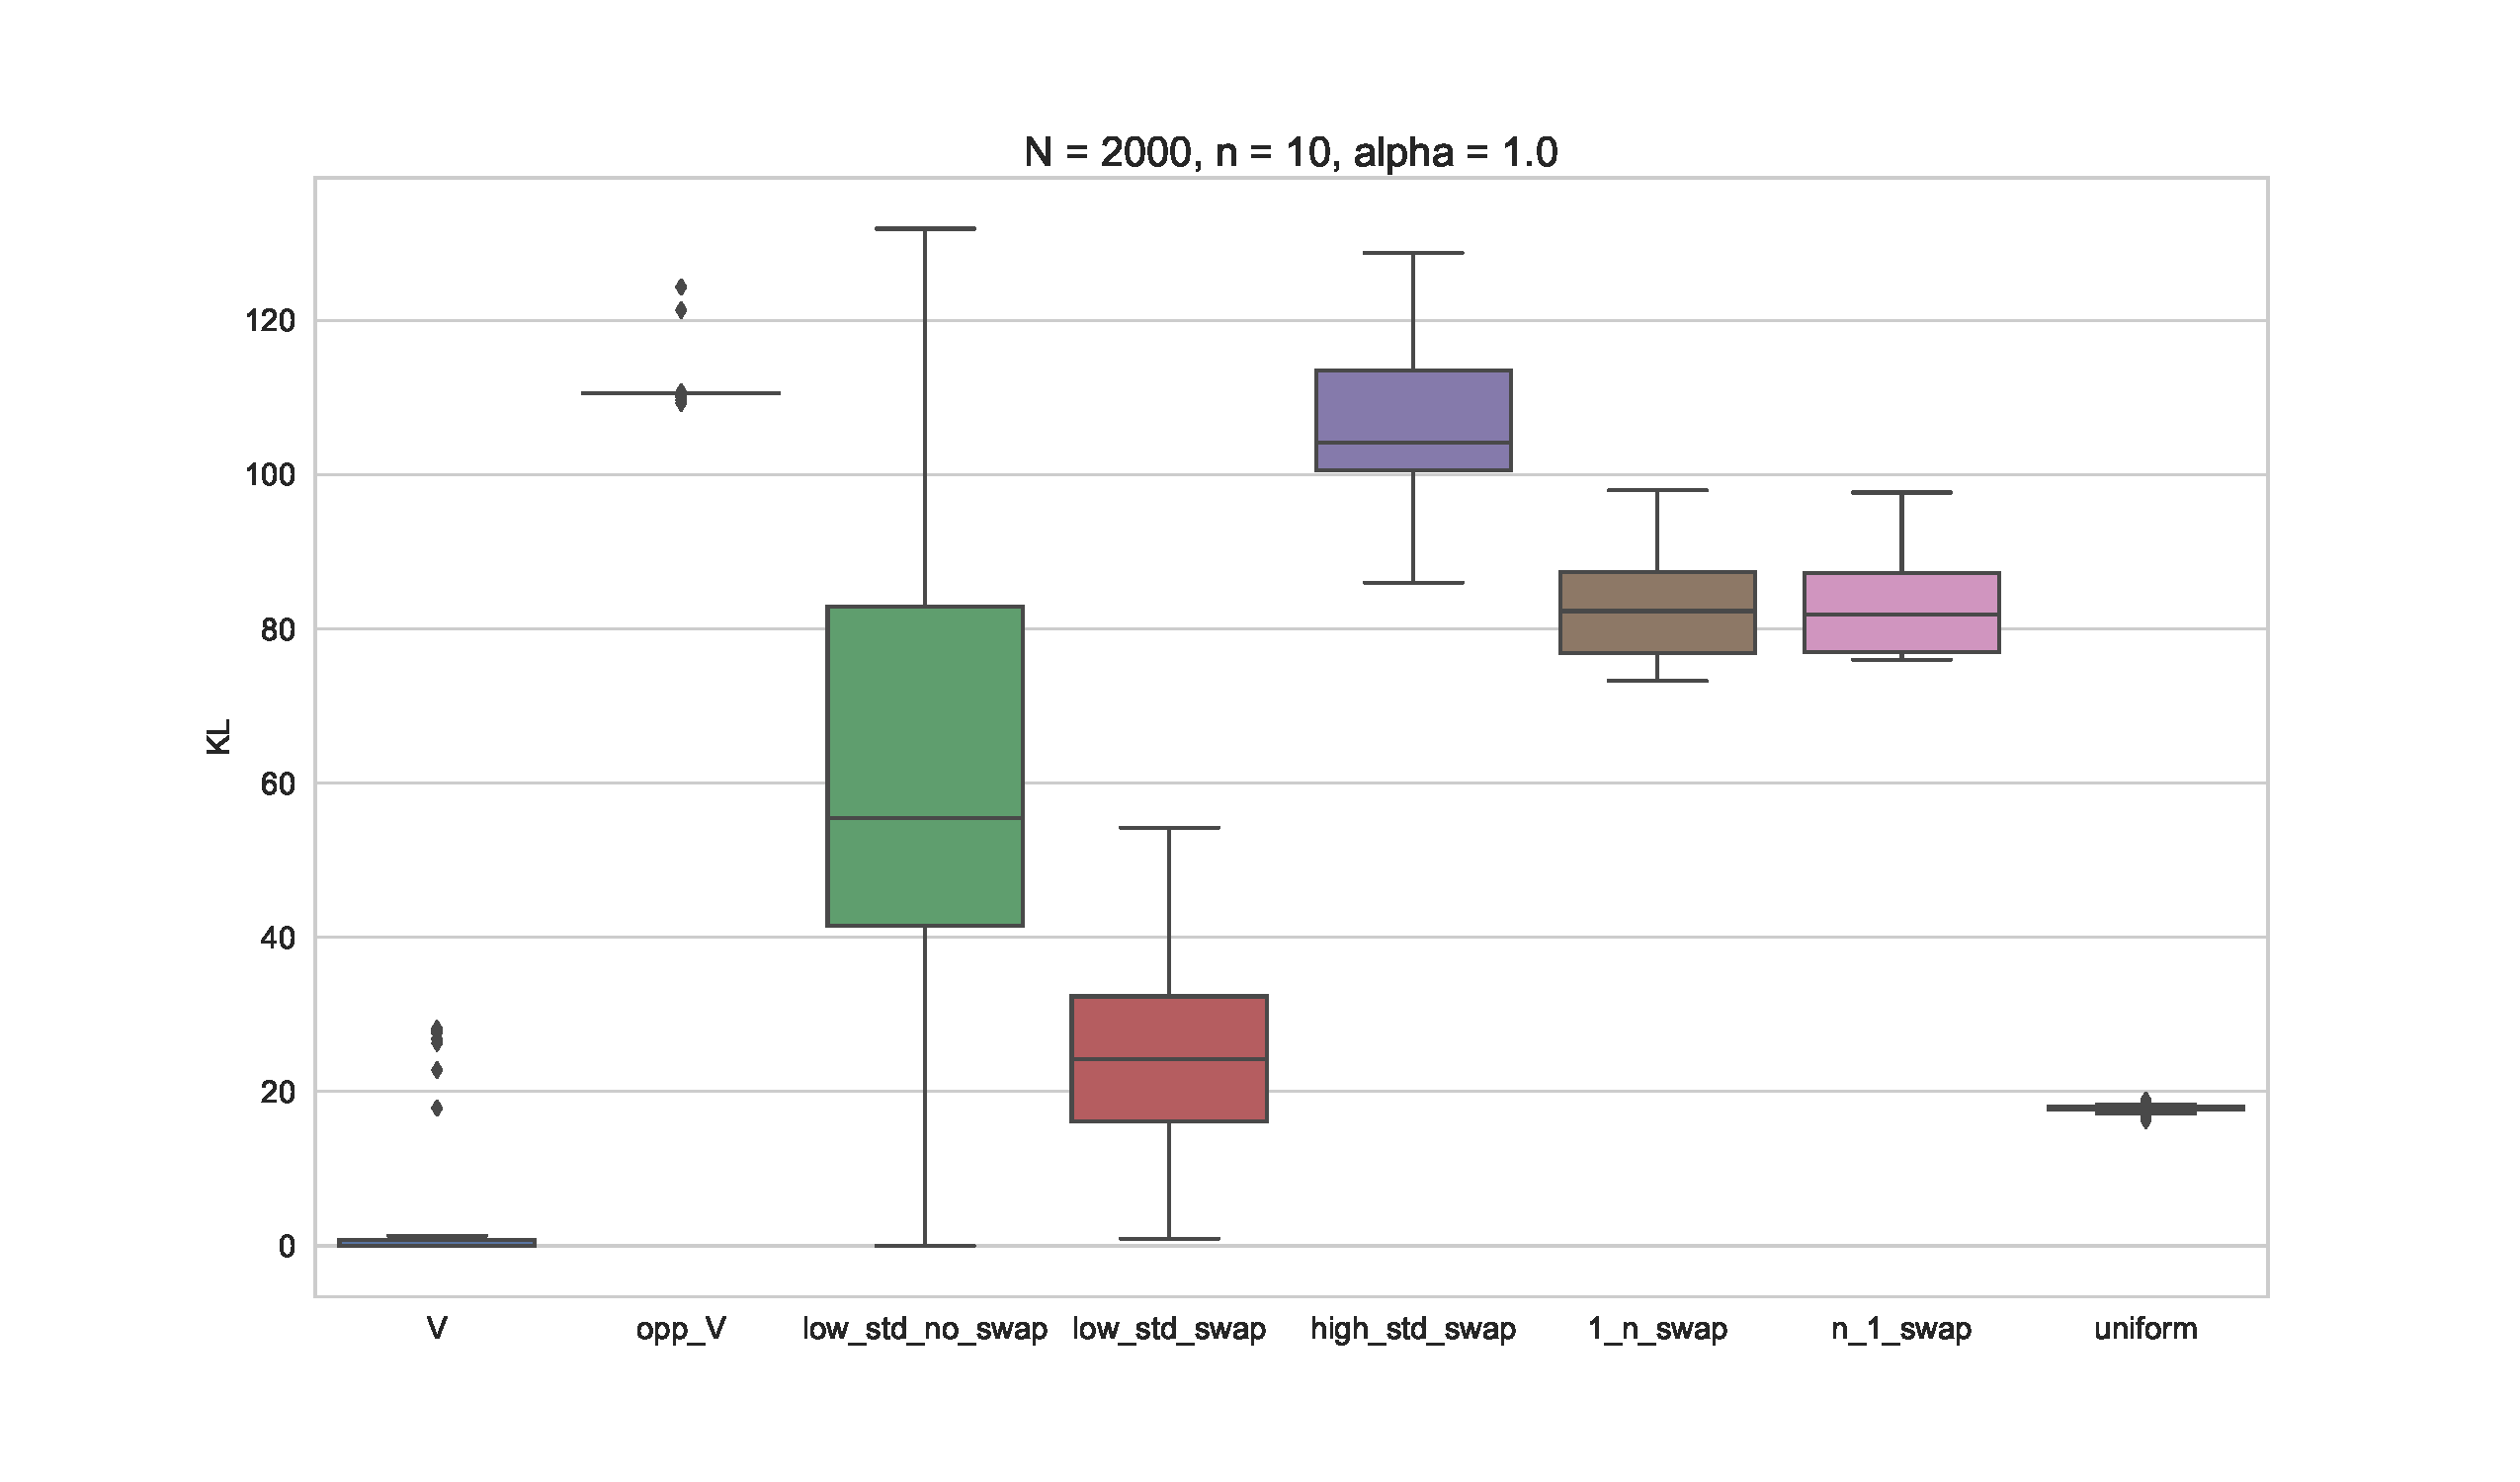
\includegraphics[width=\textwidth]{figures/theorem2_2/N2000n10alpha1.pdf}
			
		\end{minipage}
		\hfill
		\begin{minipage}[t]{.45\textwidth}
			\centering
			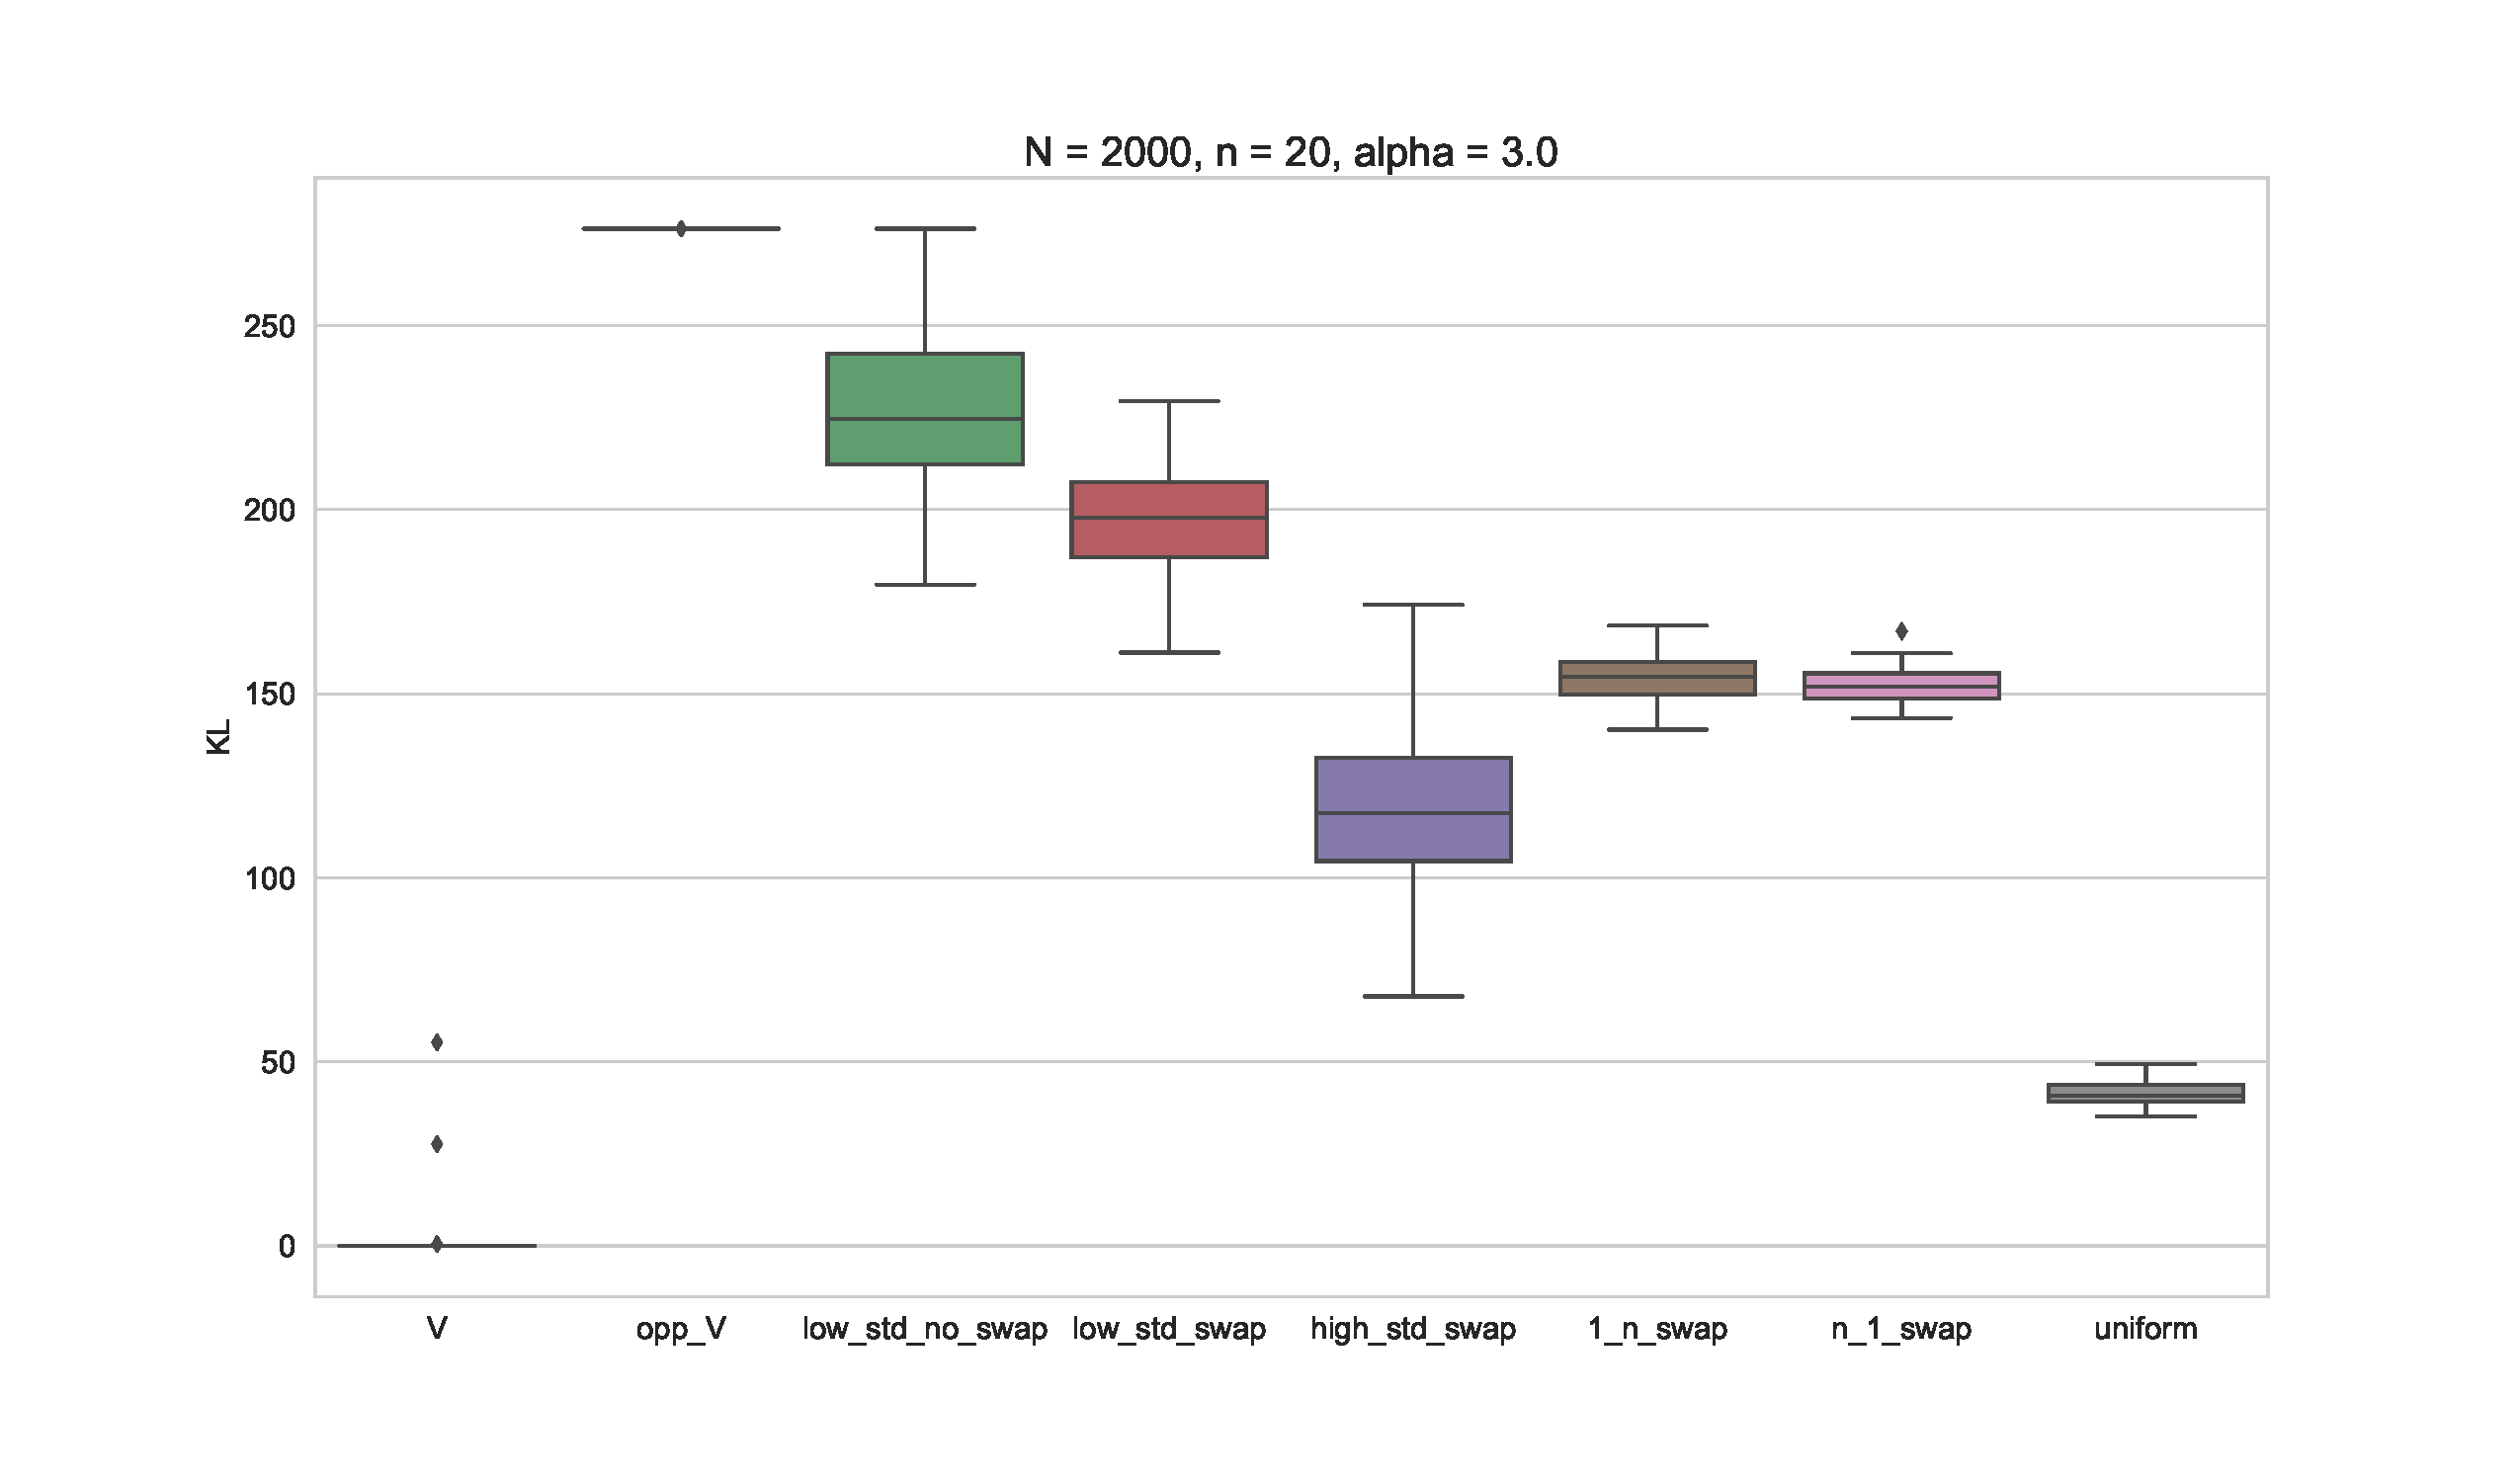
\includegraphics[width=\textwidth]{figures/theorem2_2/N2000n20alpha3.pdf}
			
		\end{minipage} 

	
	
		\begin{minipage}[t]{.45\textwidth}
			\centering
			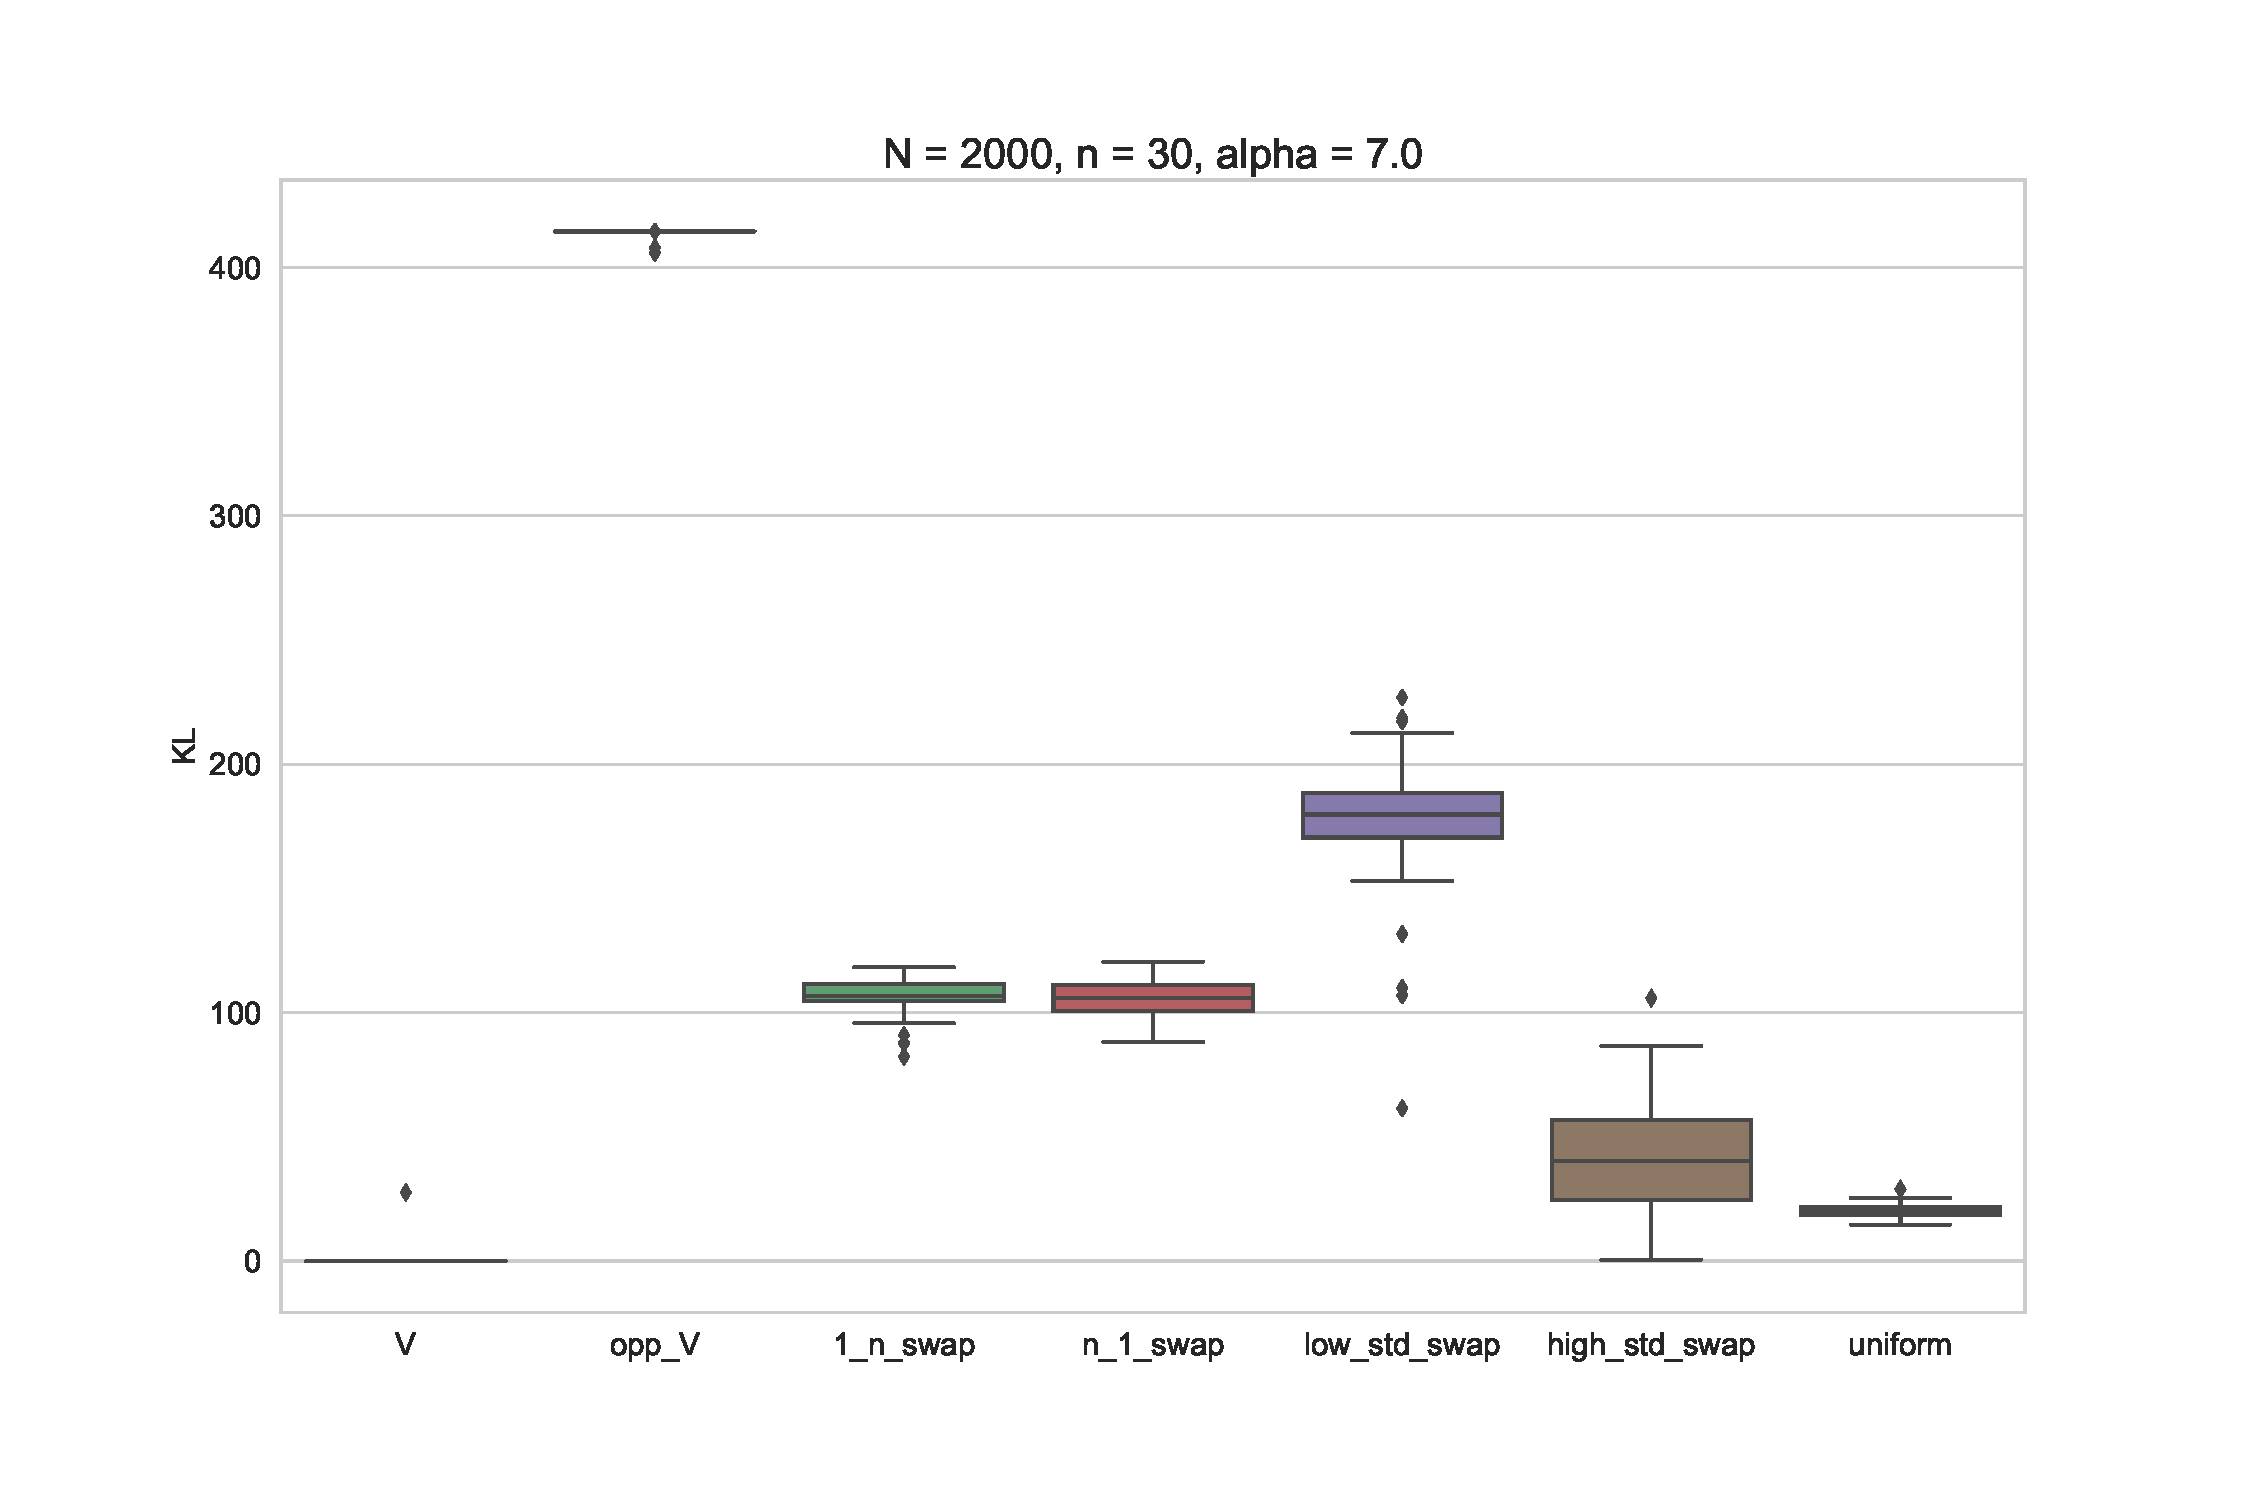
\includegraphics[width=\textwidth]{figures/theorem2_2/N2000n30alpha7.pdf}
			
		\end{minipage}
		\hfill
		\begin{minipage}[t]{.45\textwidth}
			\centering
			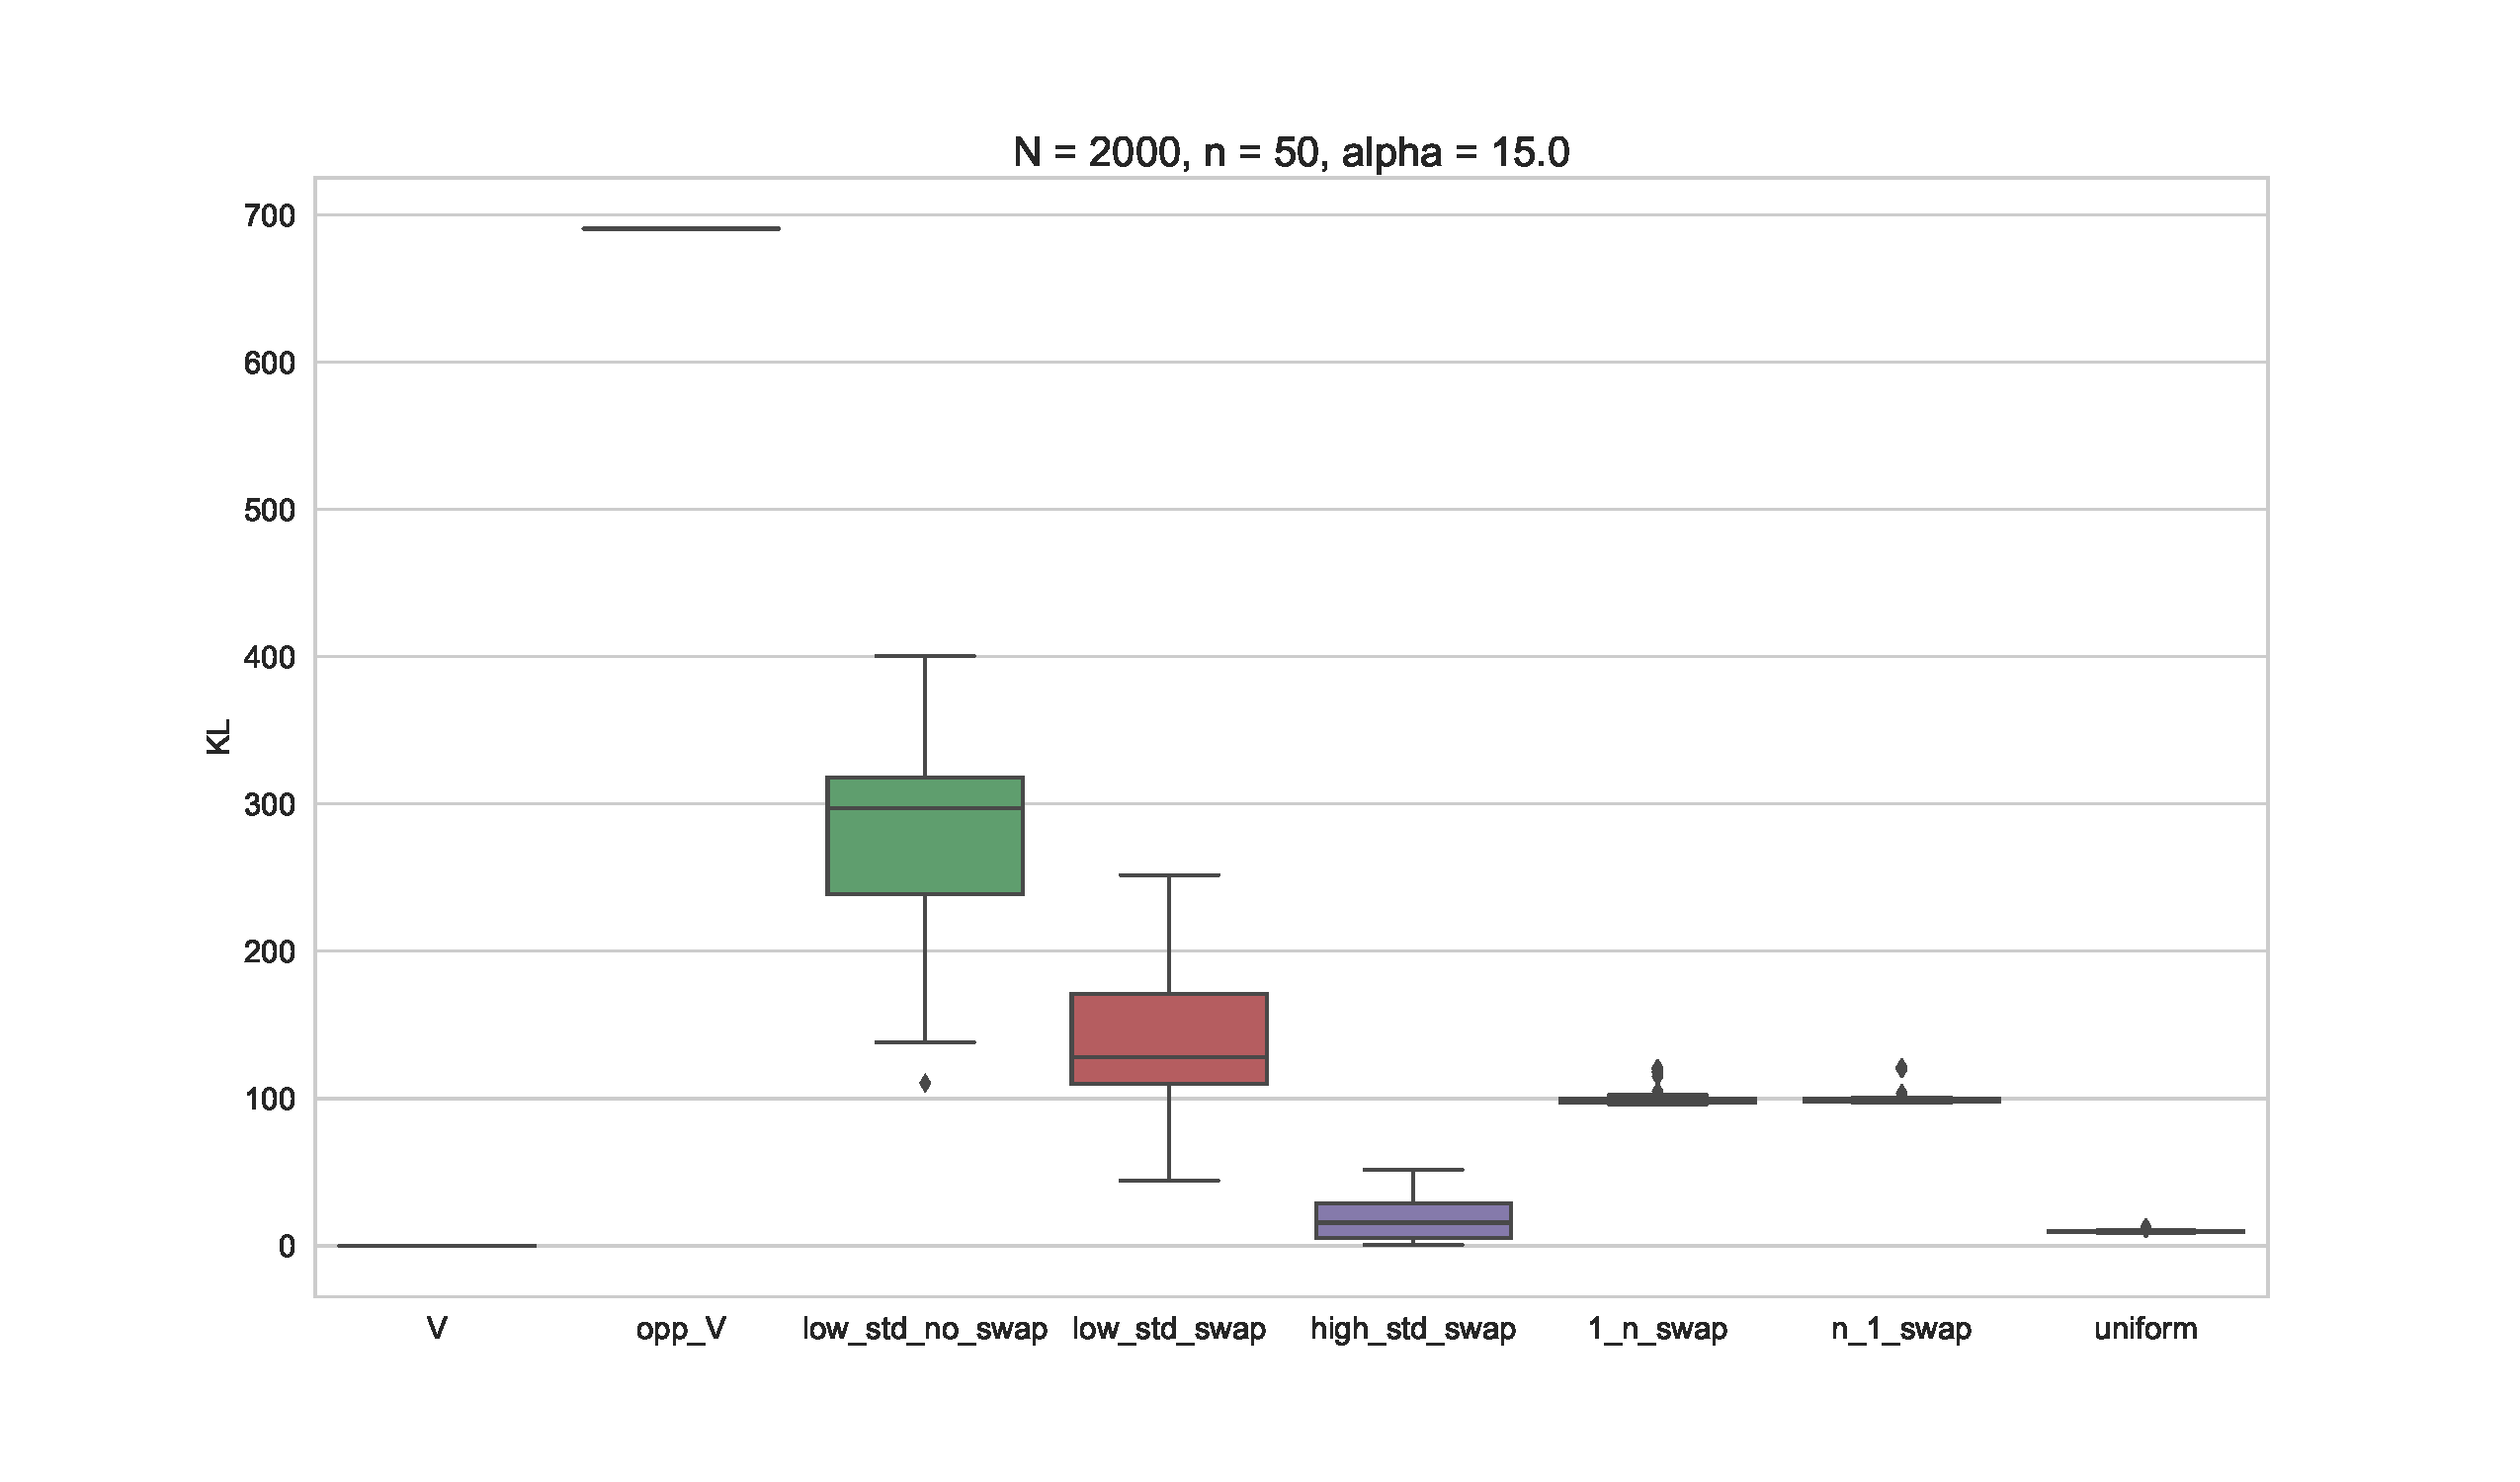
\includegraphics[width=\textwidth]{figures/theorem2_2/N2000n50alpha15.pdf}
			
		\end{minipage} 
	
	
	\caption{Comparison of KL-divergence when different choices of $g(i_1, ...,i_n|\bm{\rho}^0)$ is used. }
	\label{fig:boxPlots}
\end{figure}

Some selected heat plots are shown in \textbf{Figure}\ref{fig:heatPlot_comparison_g}. It can be clearly observed that the V-ranking is the optimal choice here. 
\begin{figure}[h!]

		\begin{minipage}[t]{.45\textwidth}
			\centering
			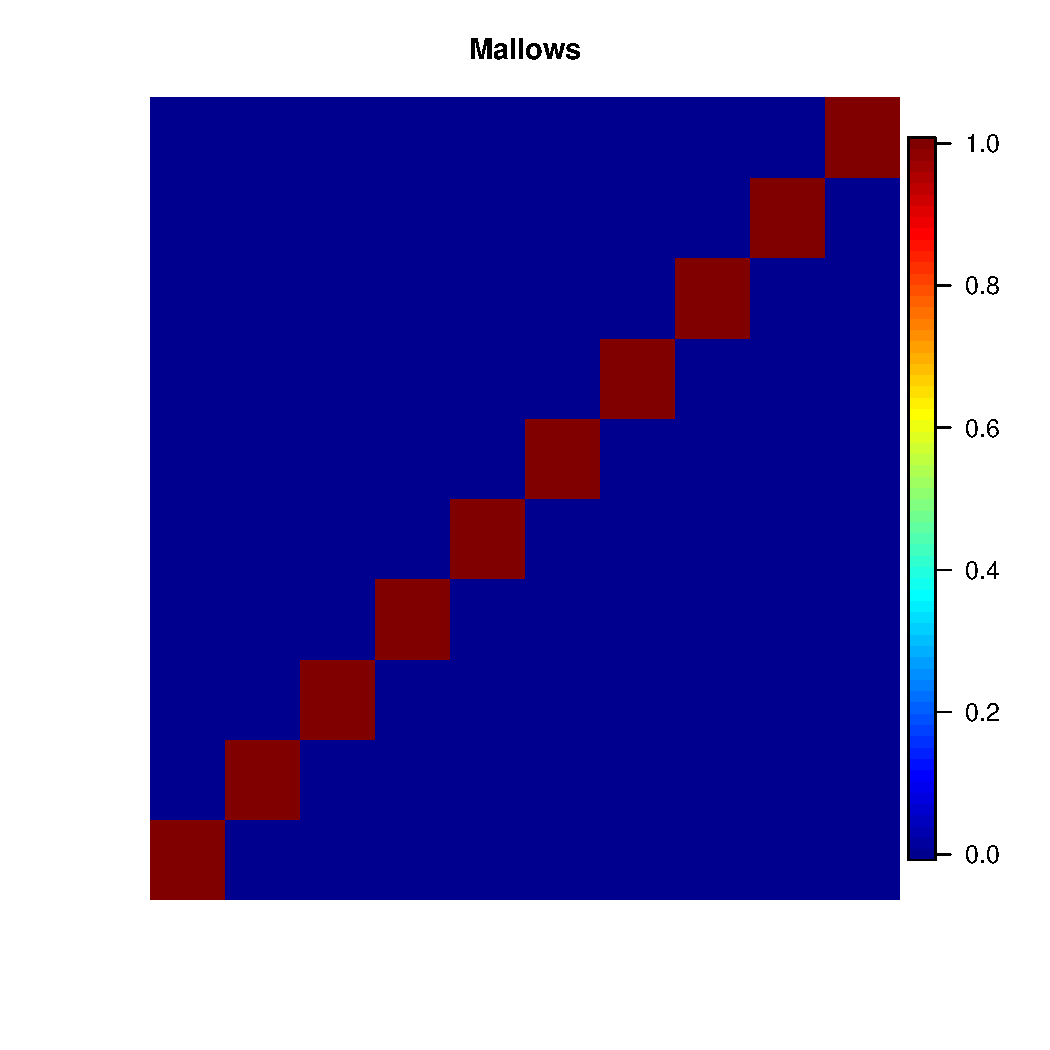
\includegraphics[width=\textwidth]{figures/theorem2_2/heat_Mallows_N2000n10alpha1run1.pdf}
			
		\end{minipage}
		\hfill
		\begin{minipage}[t]{.45\textwidth}
			\centering
			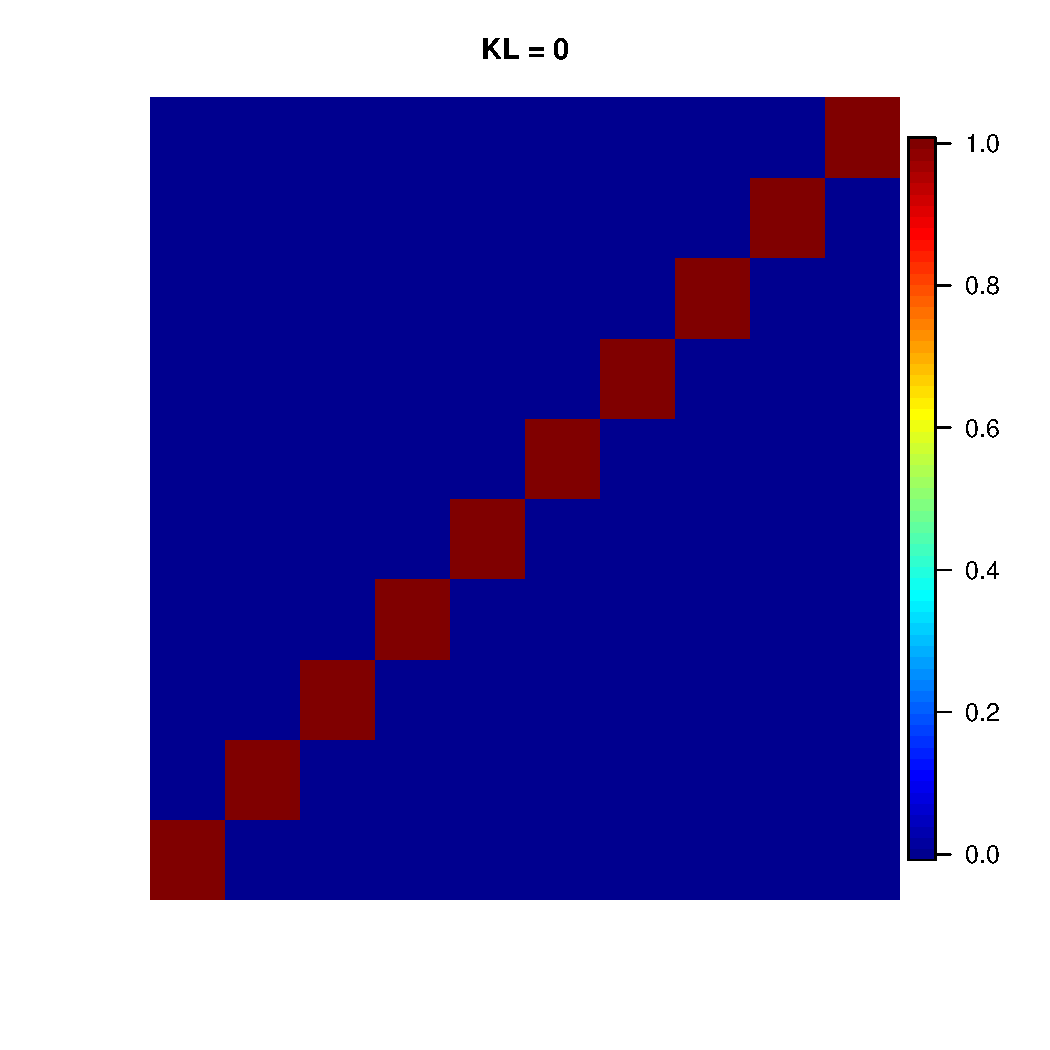
\includegraphics[width=\textwidth]{figures/theorem2_2/heat_V_N2000n10alpha1run1.pdf}
			
		\end{minipage} 
		\hfill
		\begin{minipage}[t]{.45\textwidth}
			\centering
			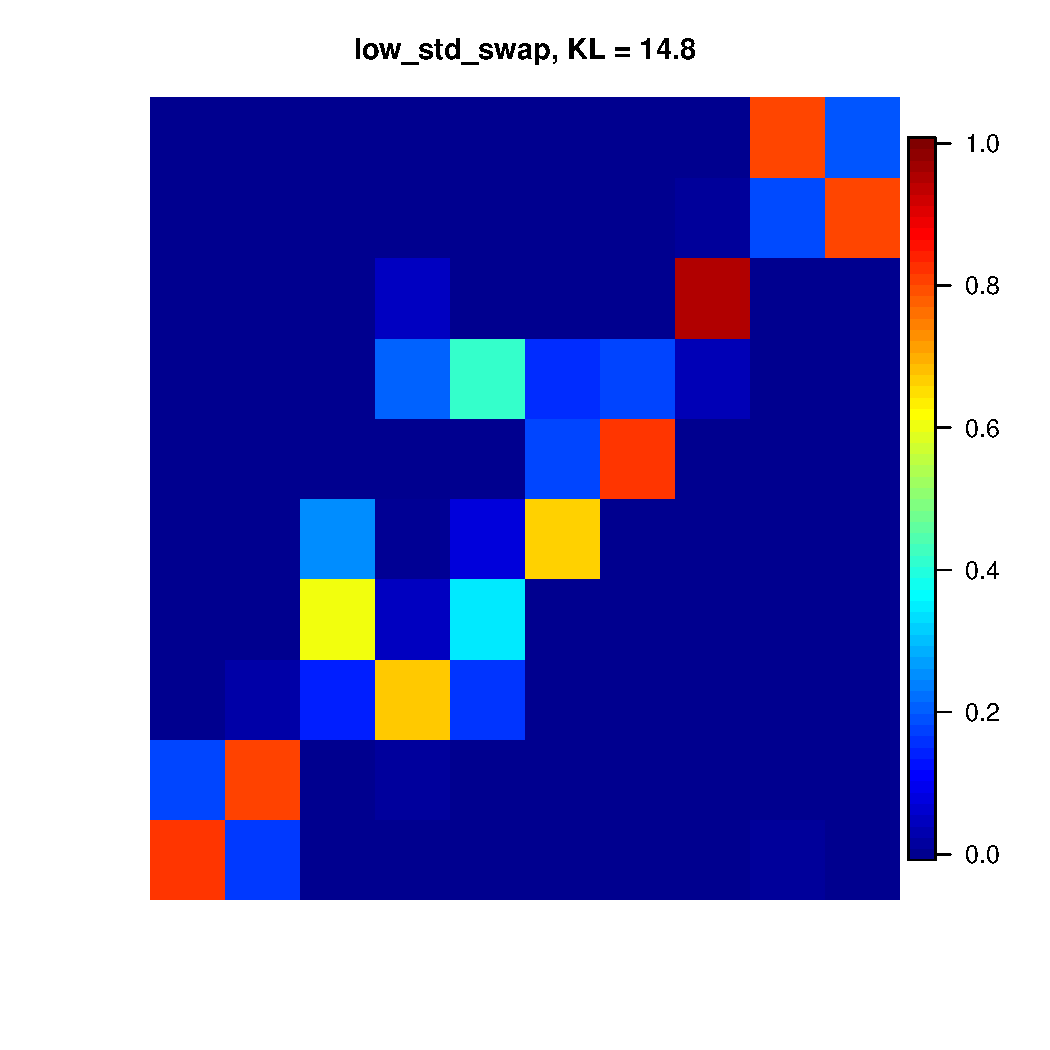
\includegraphics[width=\textwidth]{figures/theorem2_2/heat_low_std_swap_N2000n10alpha1run1.pdf}
			
		\end{minipage} 
		\hfill
		\begin{minipage}[t]{.45\textwidth}
			\centering
			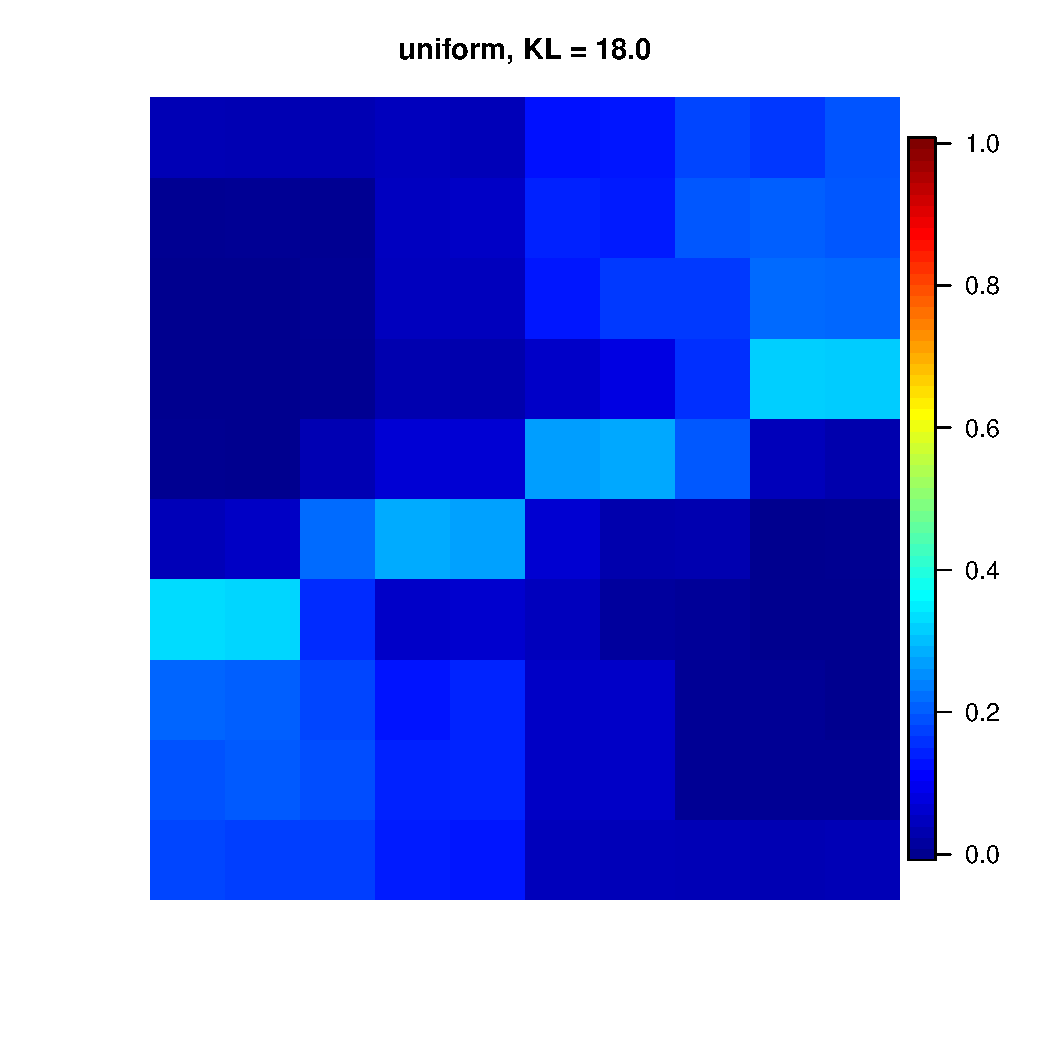
\includegraphics[width=\textwidth]{figures/theorem2_2/heat_uniform_N2000n10alpha1run1.pdf}
			
		\end{minipage} 

	\caption{Comparison of heat plots when different $g$ functions are chosen. $N = 2000, n = 10, \alpha^0 = 1$, run 1}
	\label{fig:heatPlot_comparison_g}
\end{figure}


\subsection{Evidence for Theorem \ref{theorem:gaussiannoise}}
In \textbf{Figure} \ref{fig:sigmafunction}, for each subfigure, we calculate and plot the KL-divergences between the Mallows posterior and the pseudo-likelihood, computed with different choices of $\sigma$. The left-most point on each sub-figure corresponds to the KL-divergence when no Gausian variation is introduced, i.e. $\sigma = 0$. It can be observed that for most situations shown in the figure, the lowest KL-divergence is achieved when some level of Gaussian variation is introduced, especially as $N$ and $\alpha^0$ are relatively small. However, as $N$ and $\alpha^0$ increase, the optimal $\sigma$ appears to decrease towards 0. 

\textbf{Figure} \ref{fig:heatPlot_comparison} contains a few heat plot examples. The first column are heat plots of the Mallows posterior, the middle and right columns contain heat plots of the pseudolikelihood with and without Gaussian variations. It can be observed that introducing the Gaussian variation can reduce the KL divergence between the Mallows posterior and the pseudolikelihood. This is largely due to the fact that since the true ``V-ranking'' cannot be accurately inferred from the data as $N$ is limited, we need to introduce some variation around the inferred ``V'' ranking in order to mitigate the inaccuracy.

\begin{figure}[h!]
		\subfigure[]{
		\begin{minipage}[t]{.3\textwidth}
		\centering
		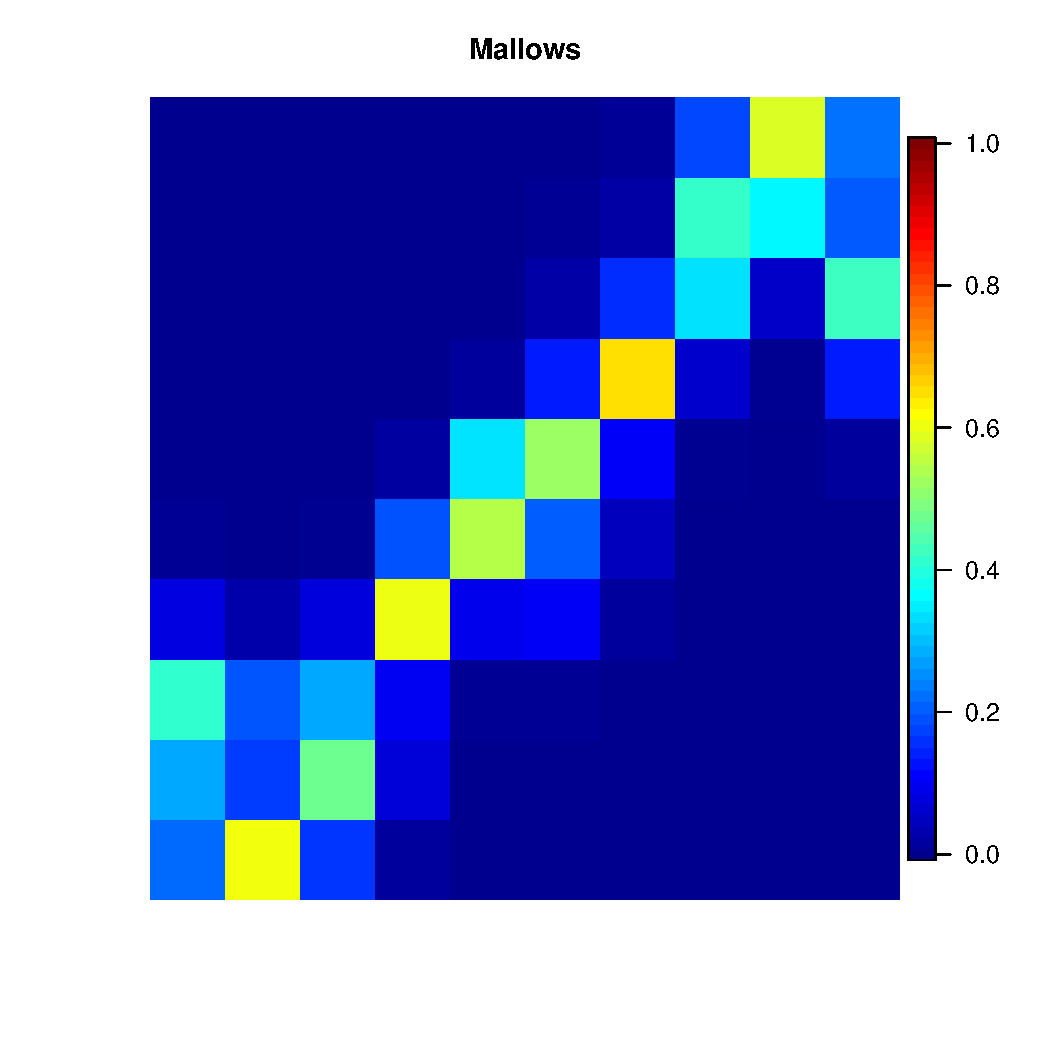
\includegraphics[width=\textwidth]{figures/Mallows_alpha1N100n10run1.pdf}
		
	\end{minipage}
	\hfill
	\begin{minipage}[t]{.3\textwidth}
		\centering
		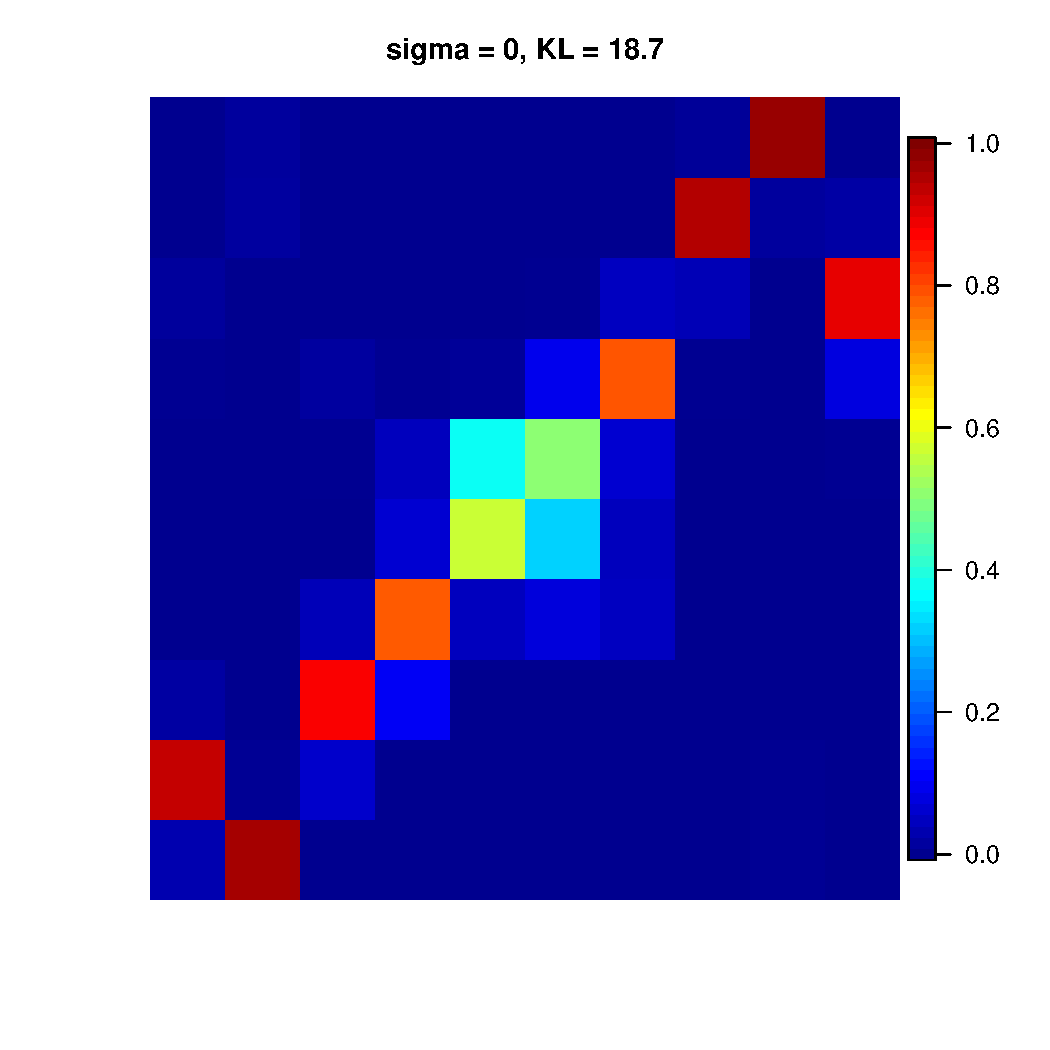
\includegraphics[width=\textwidth]{figures/Pseudo_alpha1N100n100run1sd0.pdf}

	\end{minipage} 
	\hfill
\begin{minipage}[t]{.3\textwidth}
	\centering
	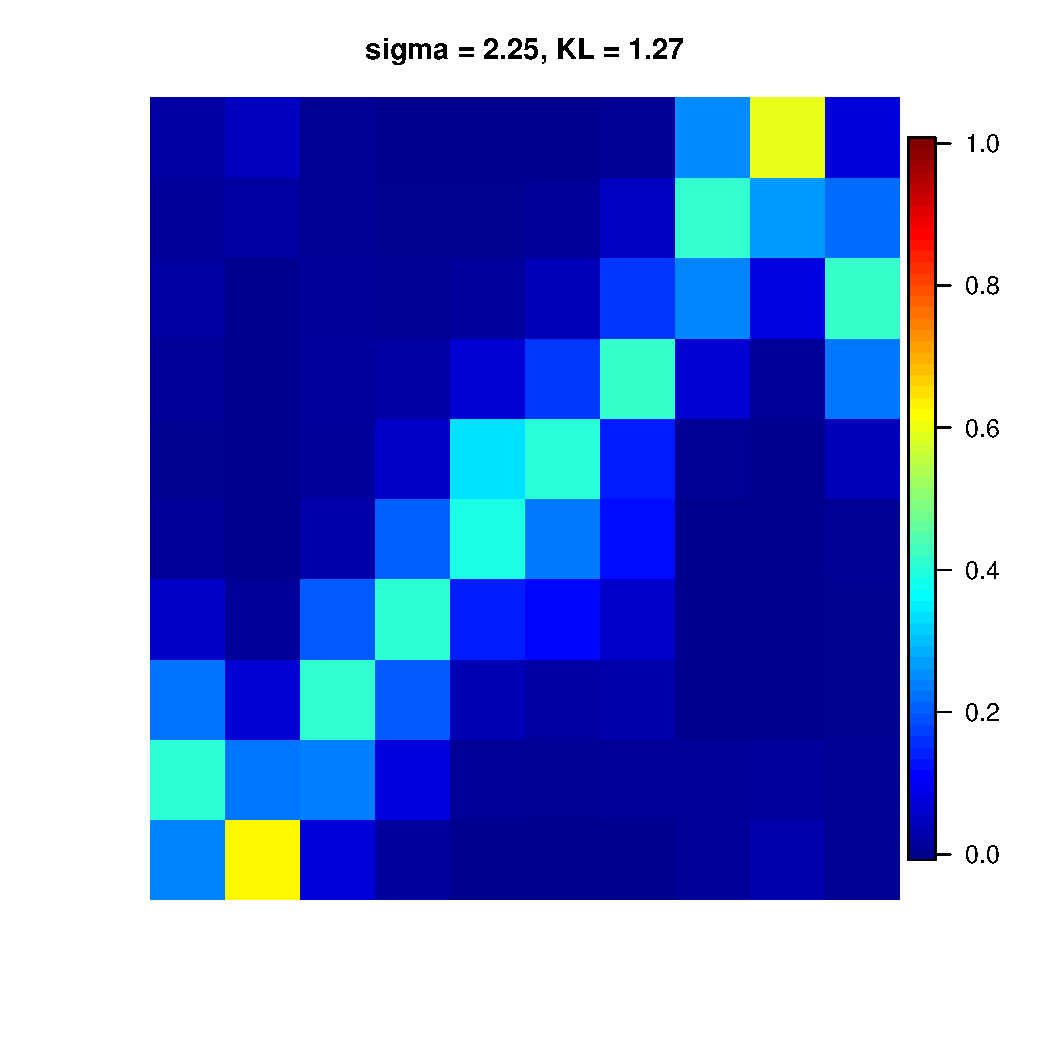
\includegraphics[width=\textwidth]{figures/Pseudo_alpha1N100n100run1sd2dot25.pdf}
	
\end{minipage} 

 }


	\subfigure[]{
		\begin{minipage}[t]{.3\textwidth}
			\centering
			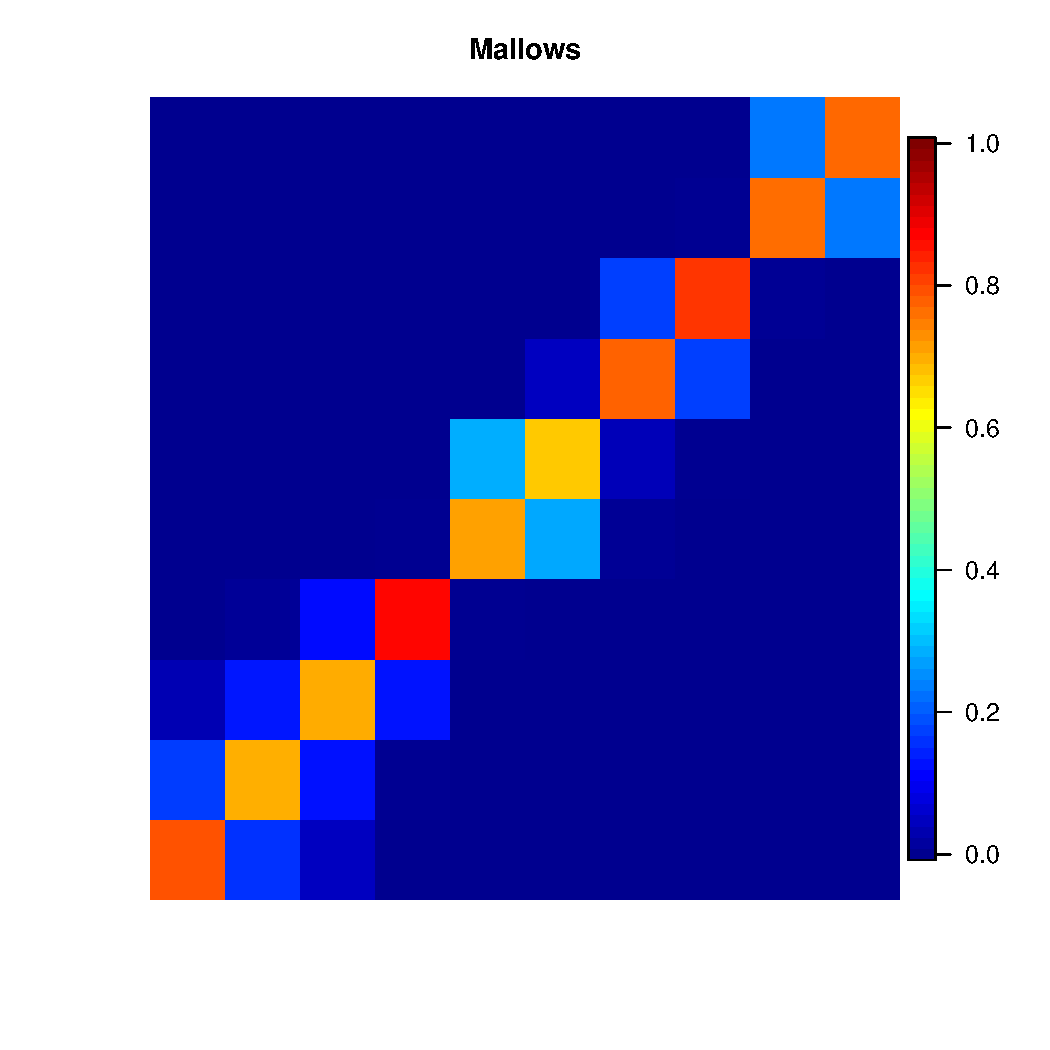
\includegraphics[width=\textwidth]{figures/Mallows_alpha1dot5N100n10run1.pdf}
			
		\end{minipage}
		\hfill
		\begin{minipage}[t]{.3\textwidth}
			\centering
			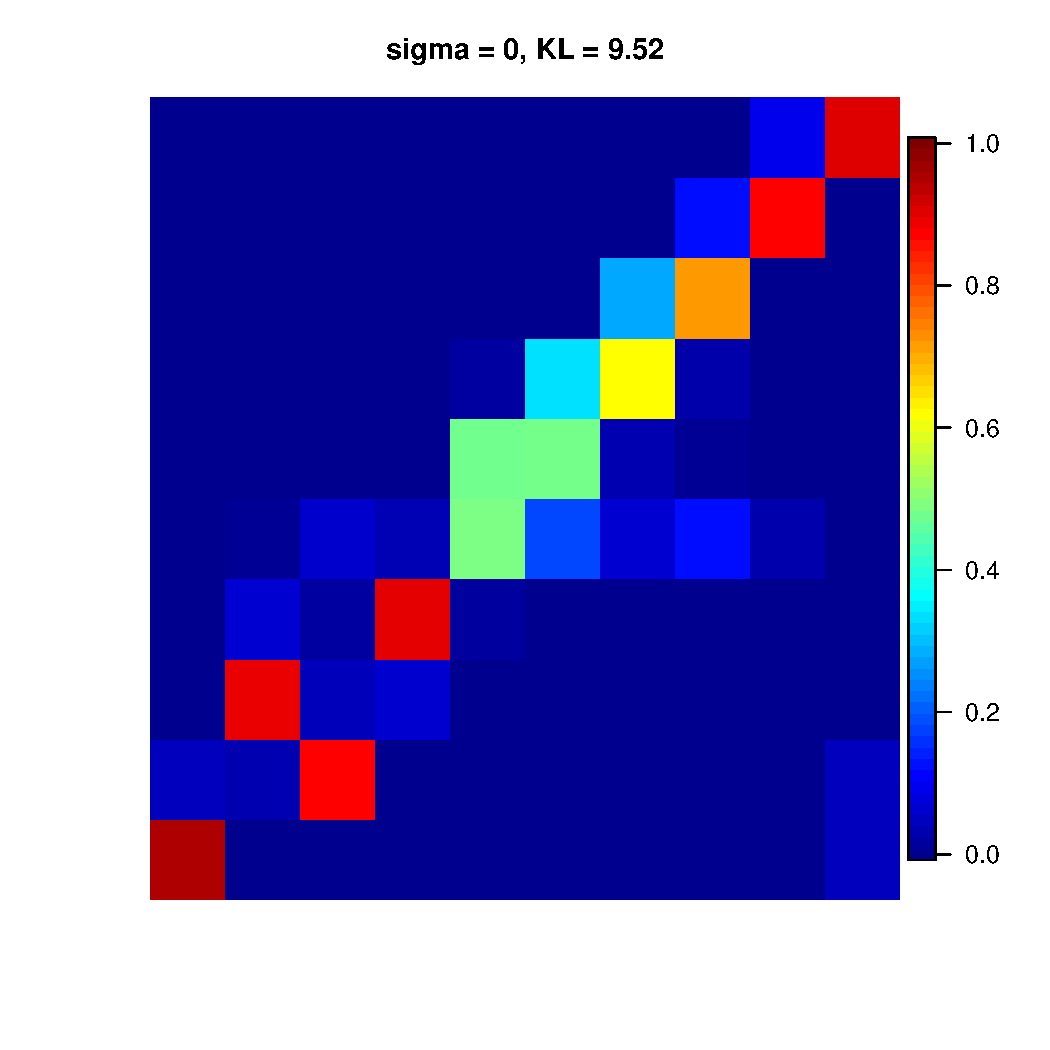
\includegraphics[width=\textwidth]{figures/Pseudo_alpha1dot5N100n100run1sd0.pdf}
			
		\end{minipage} 
		\hfill
		\begin{minipage}[t]{.3\textwidth}
			\centering
			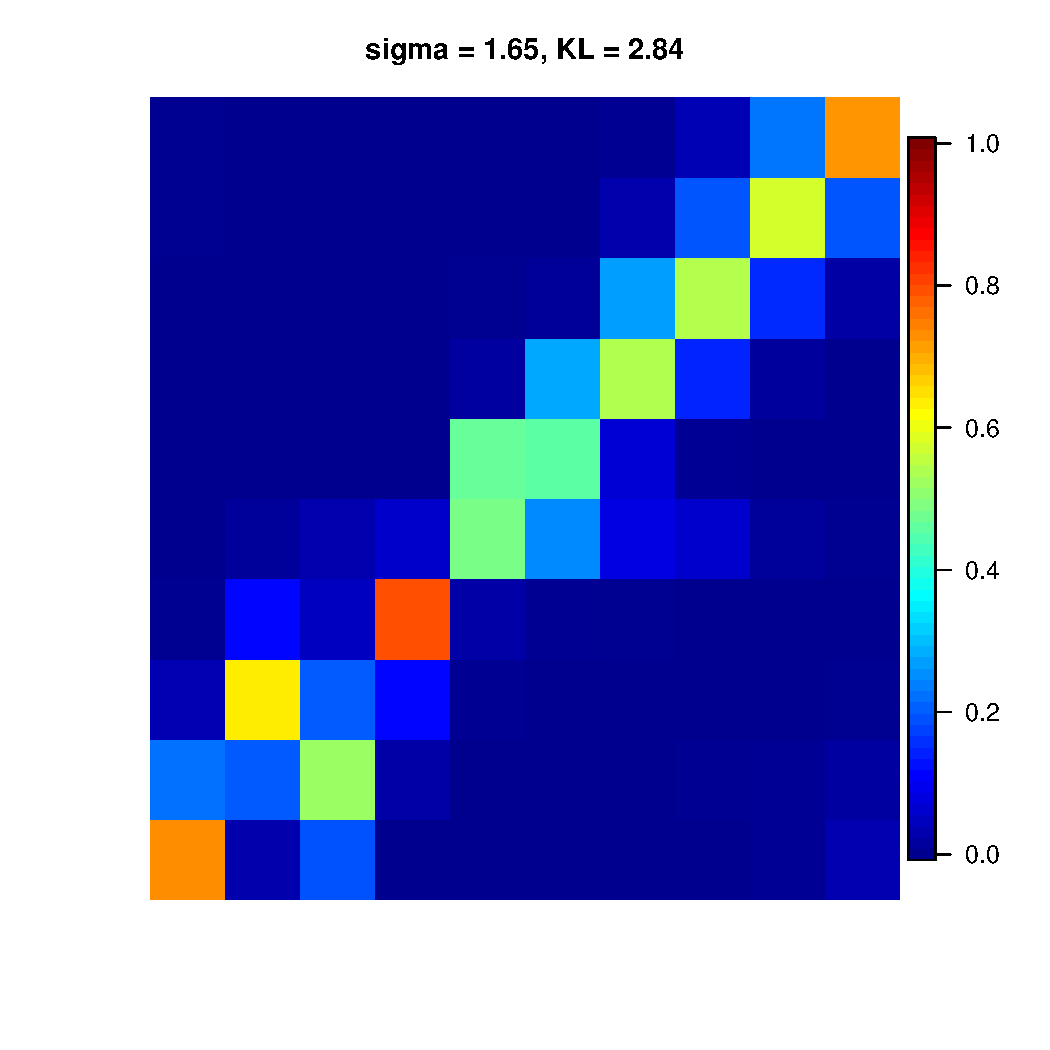
\includegraphics[width=\textwidth]{figures/Pseudo_alpha1dot5N100n100run1sd1dot65.pdf}
			
		\end{minipage} 
		
	}

\subfigure[]{
	\begin{minipage}[t]{.3\textwidth}
		\centering
		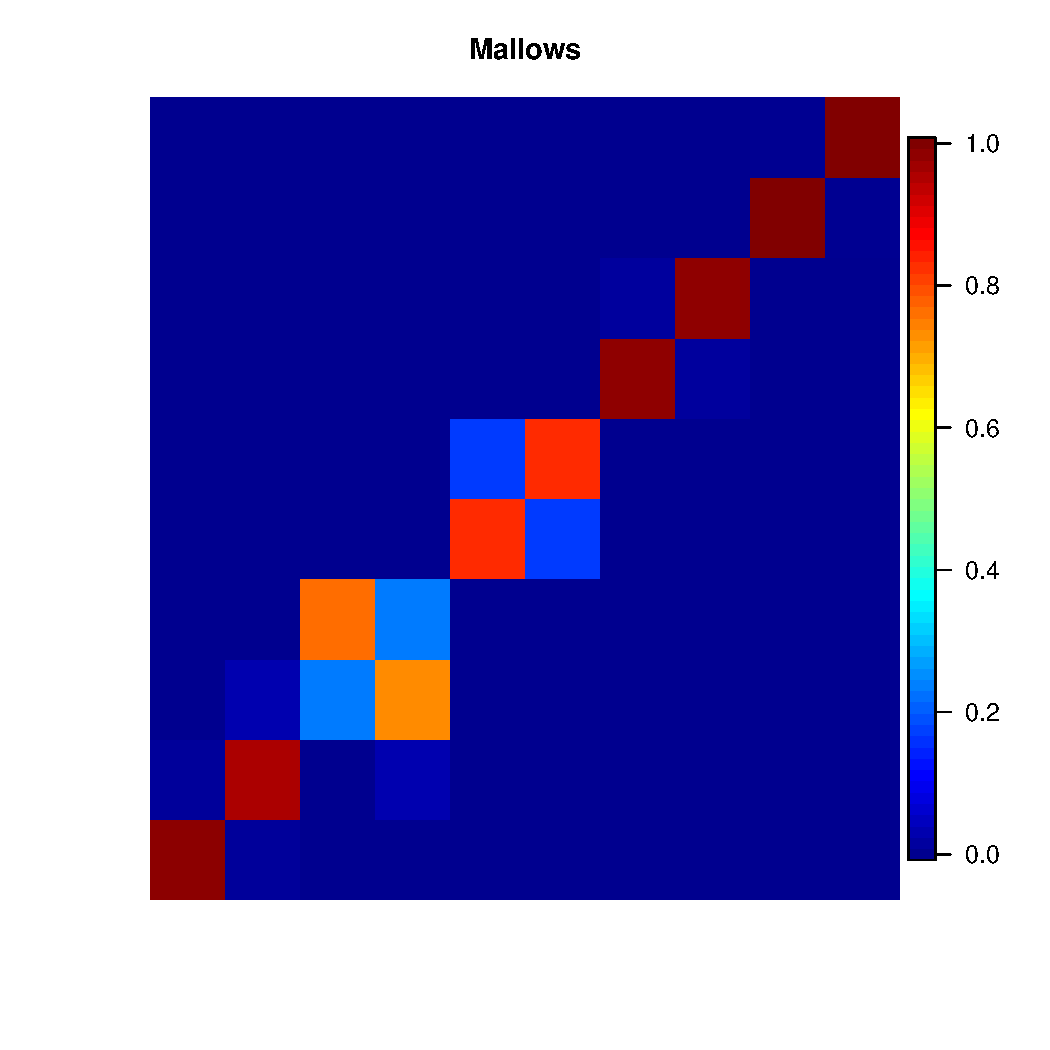
\includegraphics[width=\textwidth]{figures/Mallows_alpha2N100n10run1.pdf}
		
	\end{minipage}
	\hfill
	\begin{minipage}[t]{.3\textwidth}
		\centering
		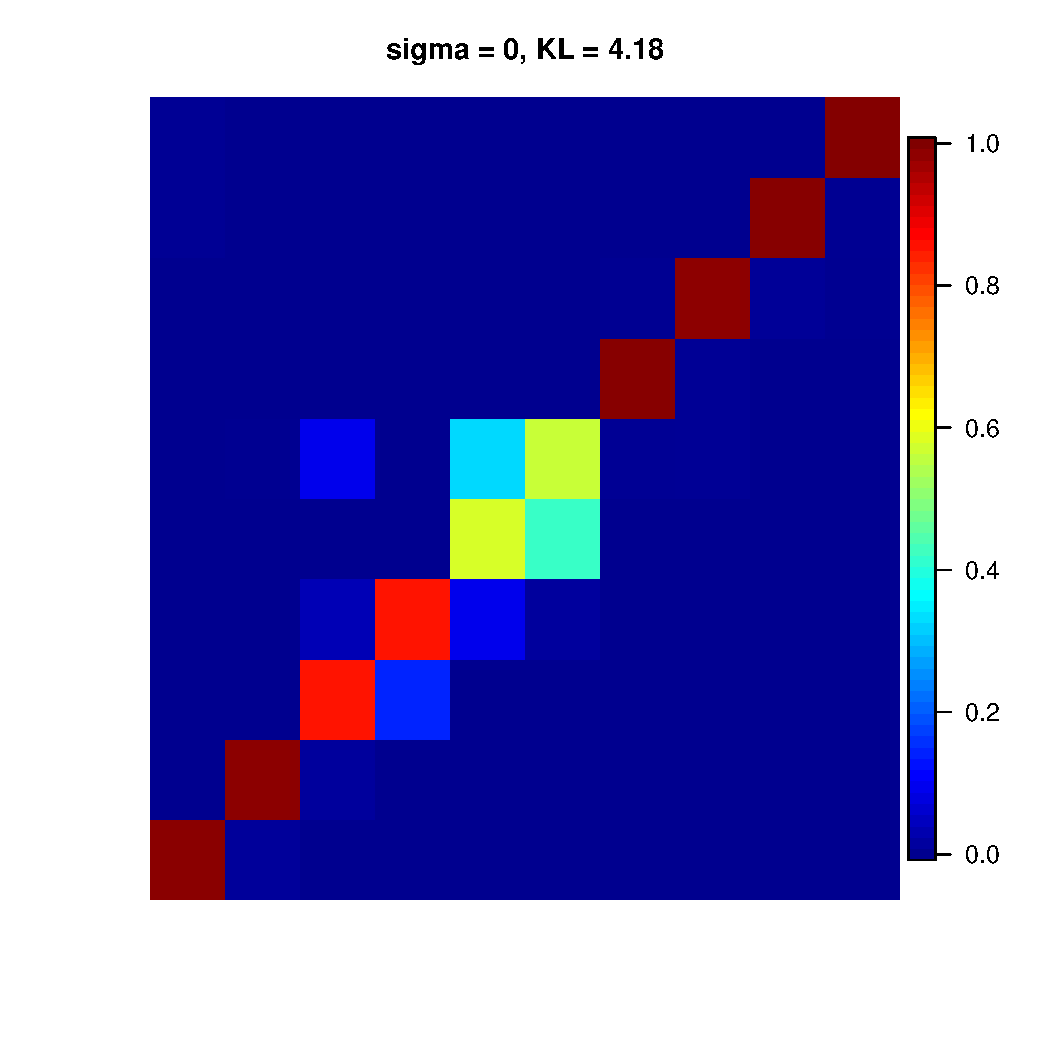
\includegraphics[width=\textwidth]{figures/Pseudo_alpha2N100n100run1sd0.pdf}
		
	\end{minipage} 
	\hfill
	\begin{minipage}[t]{.3\textwidth}
		\centering
		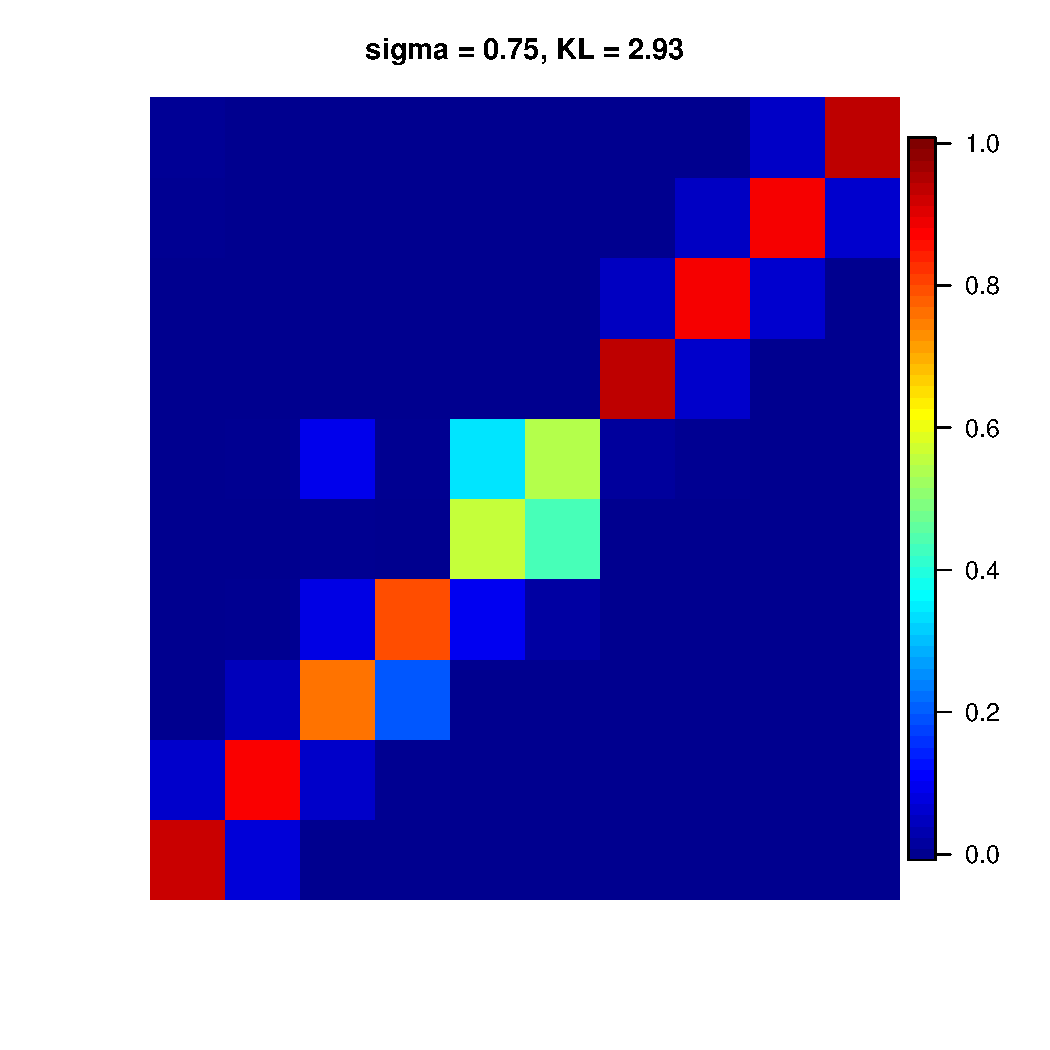
\includegraphics[width=\textwidth]{figures/Pseudo_alpha2N100n100run1sd0dot75.pdf}
		
	\end{minipage} 
	
}

	
\caption{left column: Mallows; middle column: pseudolikelihood without Gaussian variation; right column: pseudolikelihood with Gaussian variation. $N = 200, n = 10$, $\alpha^0 = 1, 1.5, 2$ respectively, from top to bottom}
\label{fig:heatPlot_comparison}
\end{figure}
\subsection{Evidence for Theorem \ref{theorem:sigmafunction}}

\subsubsection{Optimal $\sigma$ is determined by $N, n, \alpha^0$}
As shown in \textbf{Figure} \ref{fig:sigmafunction}, in each subfigure, the $\sigma$ value that corresponds to the lowest KL-divergence is the optimal $\sigma$ for its specific ($N, n, \alpha^0$) set up. Each row of 3 figures shows a comparison of the optimal $\sigma$ when one of the variables ($N$, $n$, $\alpha$) changes. It can be observed that all three variables have an impact on the optimal value of $\sigma$. More specifically, the optimal choice of $\sigma$ appear to decrease as $N$ and $\alpha^0$ increase, and as $n$ decreases.
\begin{figure}[h!]
	\subfigure[]{
	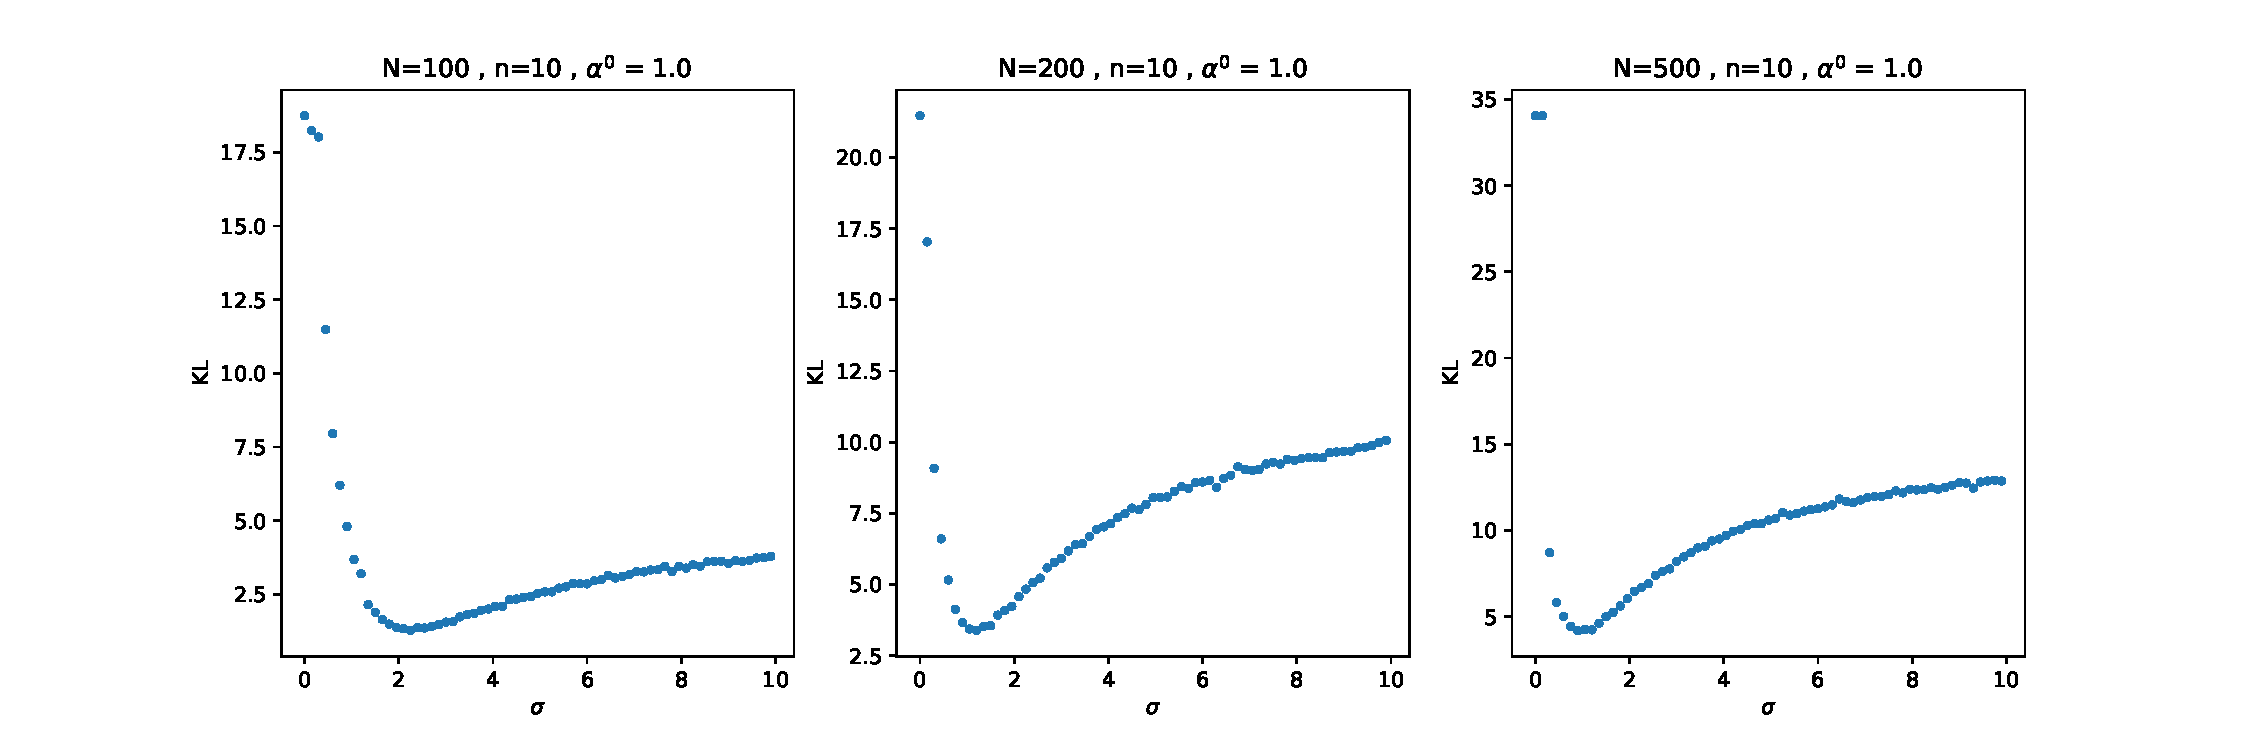
\includegraphics[width=\linewidth]{figures/diff_N_users.pdf}\label{fig_diff_user}}
	\subfigure[]{
	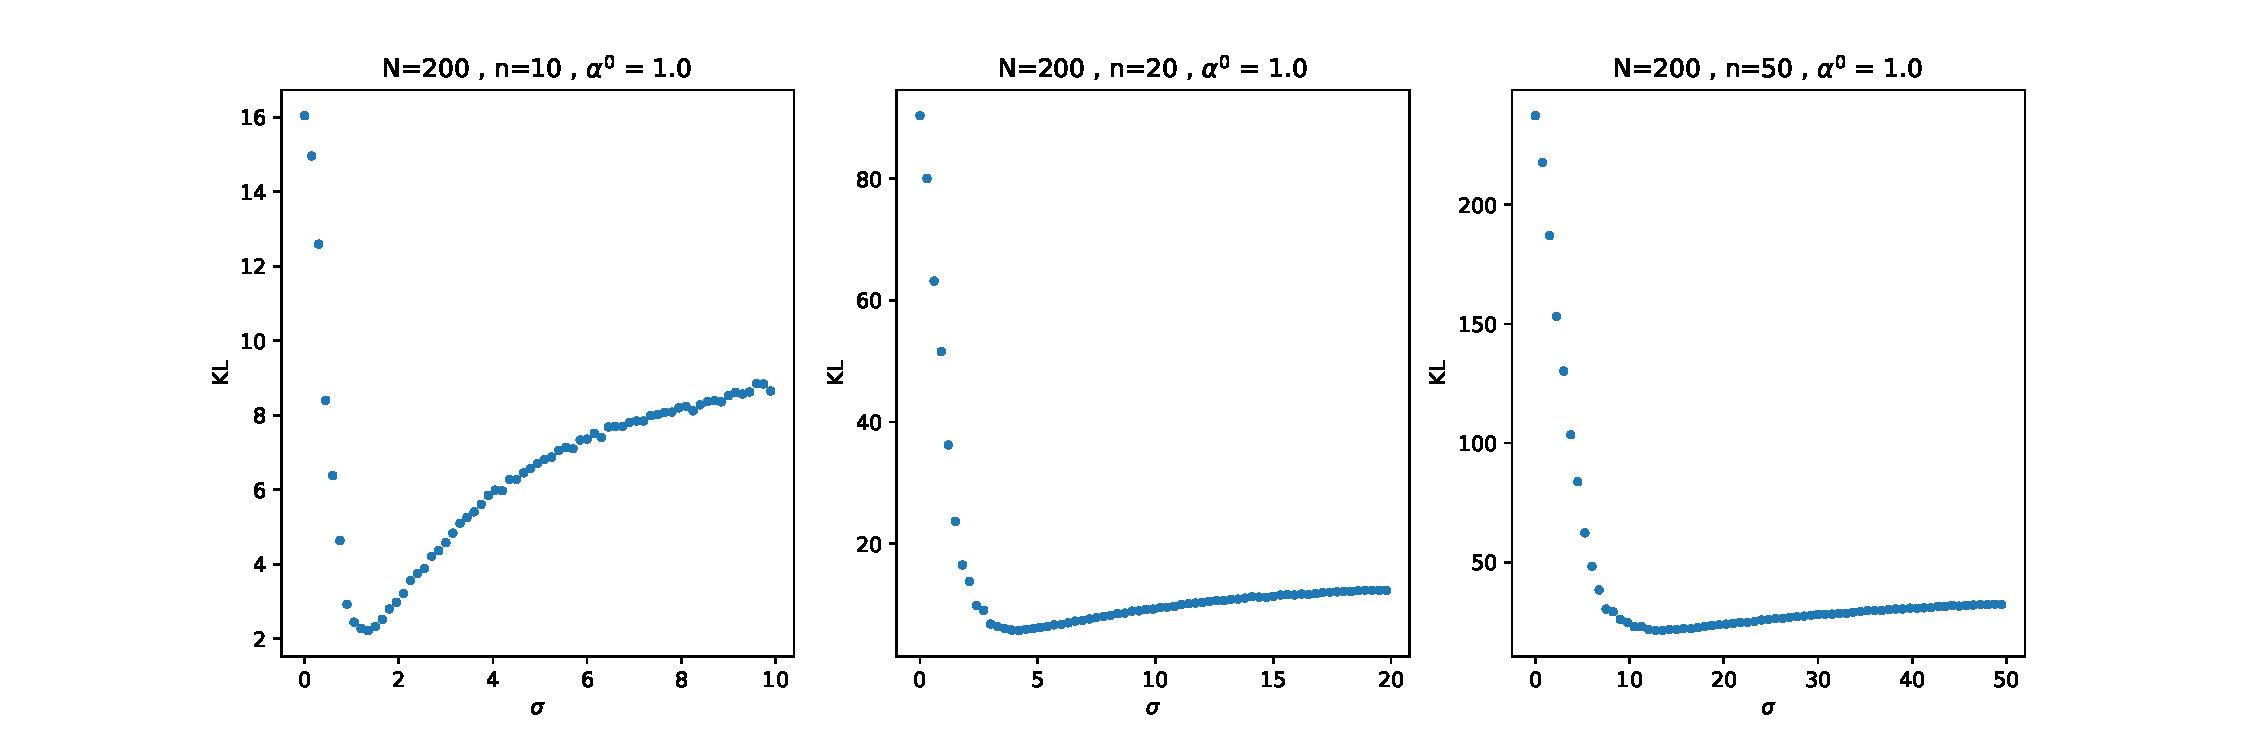
\includegraphics[width=\linewidth]{figures/diff_n.pdf}\label{fig_diff_n}}
	\subfigure[]{
	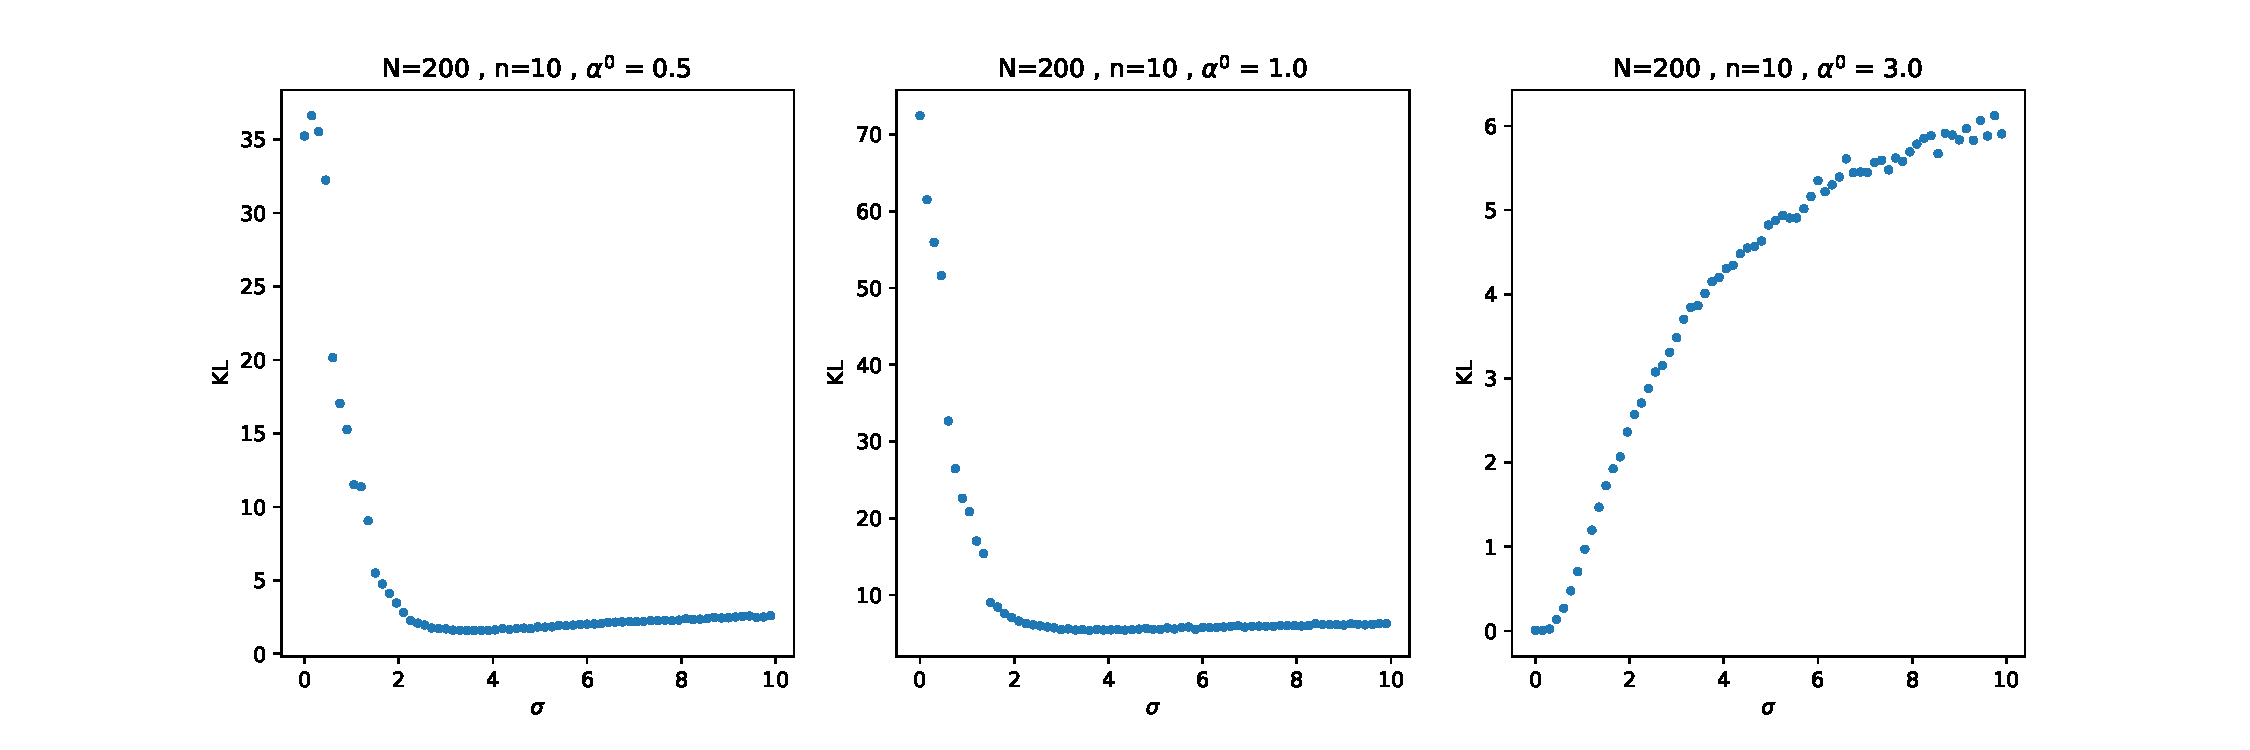
\includegraphics[width=\linewidth]{figures/diff_alpha.pdf}\label{fig_diff_alpha}}
\caption{x-axis: $\sigma$, y-axis: KL-divergence}
\label{fig:sigmafunction}
\end{figure}

For each $N$, $n$ and $\alpha^0$, we simulate 10 datasets, and for each dataset, a grid of $\sigma$ values are tried out. In \textbf{Figure }\ref{fig:optimSigma}, we plot $\alpha^0$ on the x-axis, and its corresponded optimal $\sigma$ on the y-axis. It can be observed that when $\alpha^0$ and $N$ are large, and $n$ is small, all $\sigma$ values result in small KL-divergence. To simplify, in these situations, we can safely set $\sigma = 0$ to achieve small KL-divergence. As $N$ and $\alpha^0$ decreases and as $n$ increases, optimal $\sigma$ increases.
\begin{figure}[h!]
		\subfigure[]{
		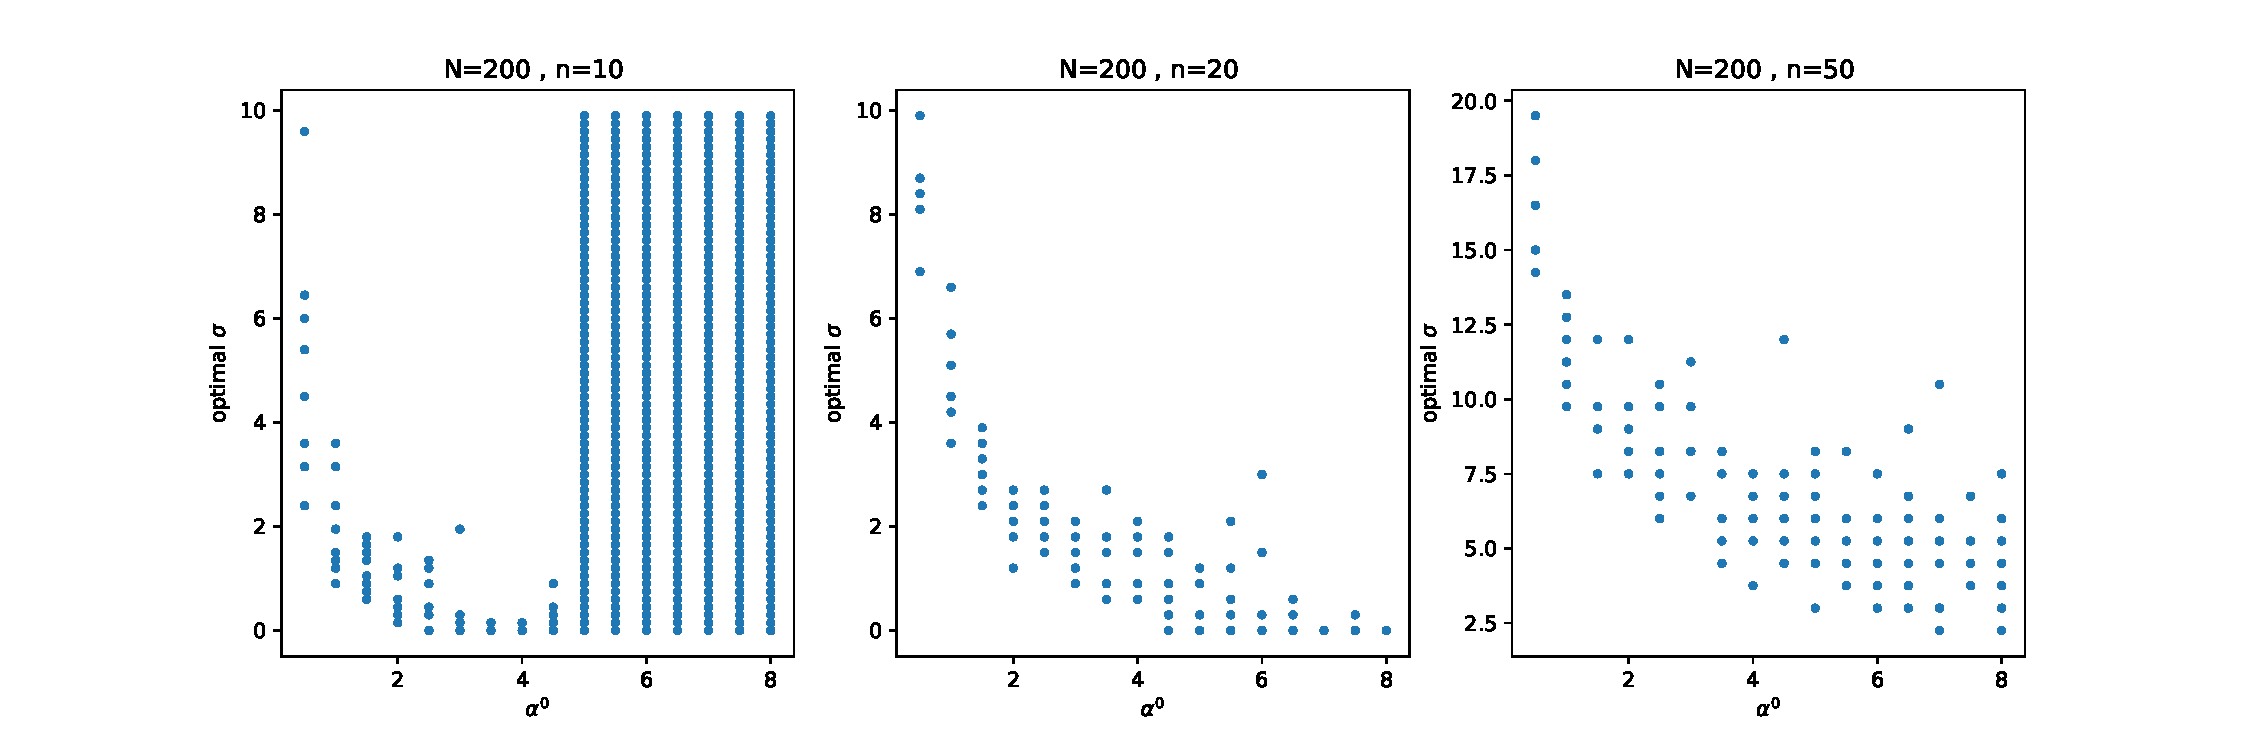
\includegraphics[width=\linewidth]{figures/2_4_sameN200diffn.pdf}\label{fig_optimSigma_diff_n}}
		\subfigure[]{
		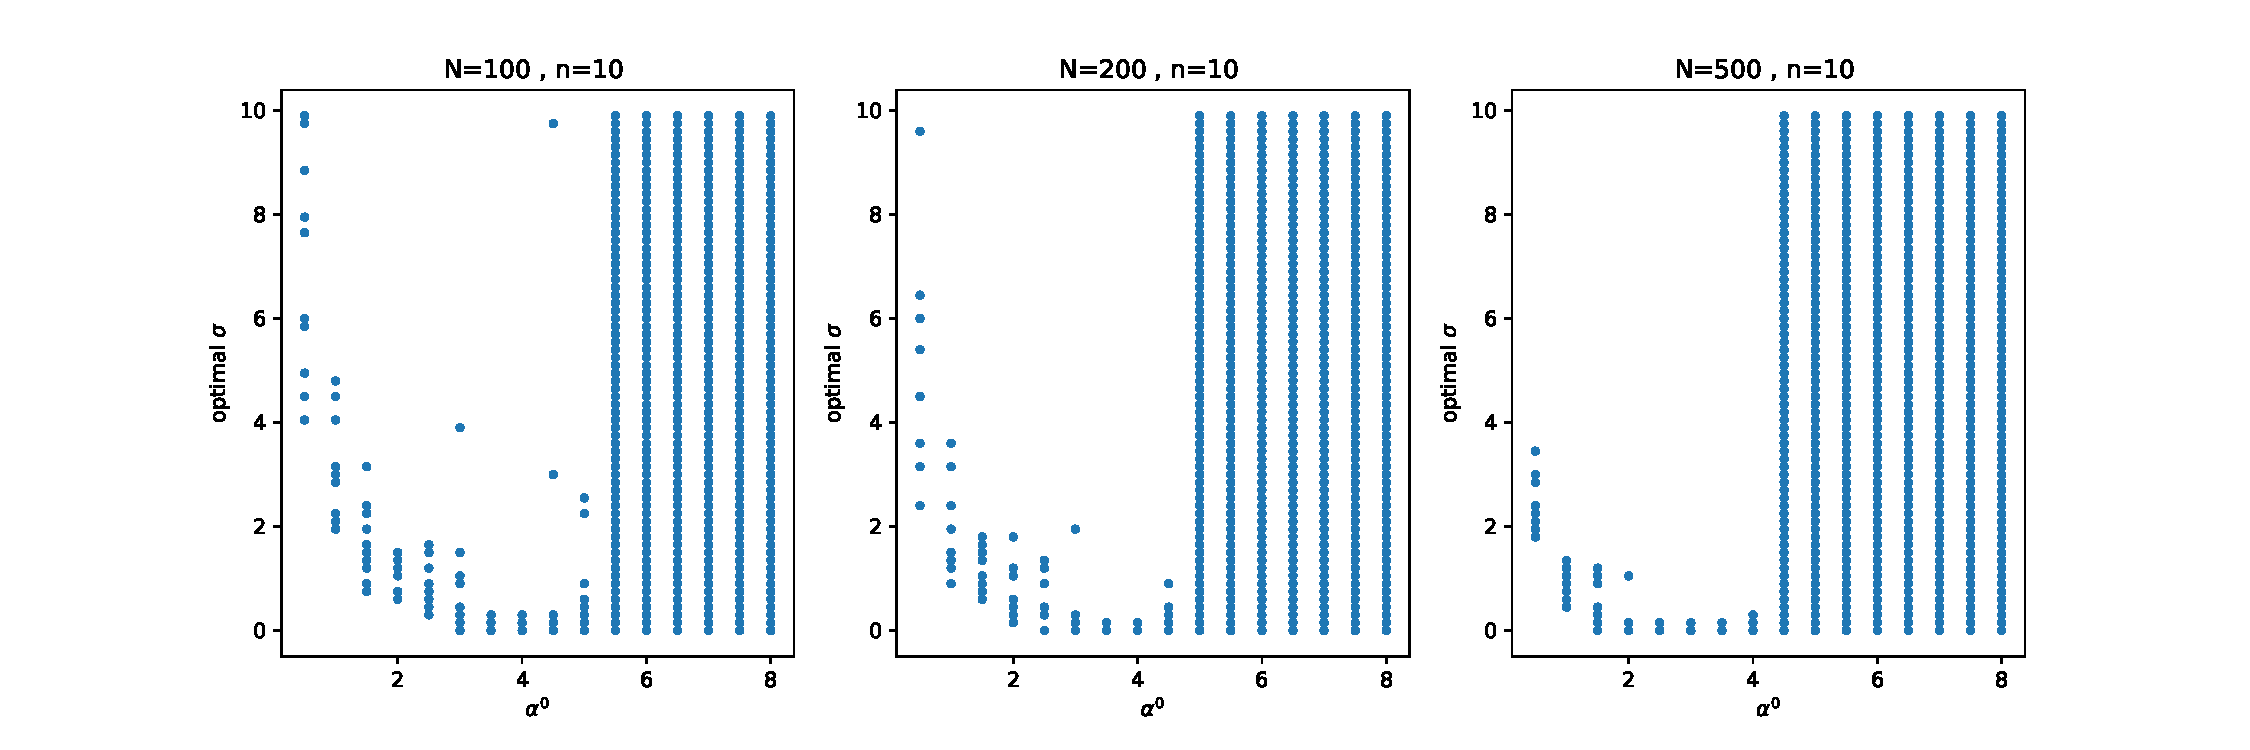
\includegraphics[width=\linewidth]{figures/2_4_samen10diffN.pdf}\label{fig_optimSigma_diff_N}}
		\caption{x-axis: $\alpha^0$, y-axis: optimal $\sigma$}
		\label{fig:optimSigma}
\end{figure}

\subsubsection{Using data standard deviation / n as a proxy for $\alpha^0$}
Under most situations, the value of $\alpha^0$ is unknown, however, we can compute the marginal standard deviation of each item from the data, and normalize it by deviding it by n. The trend demonstrated in \textbf{Figure }\ref{fig:optimSigma} is well-preserved, as shown in \textbf{Figure }\ref{fig:optimSigma_sd_data}.

\begin{figure}[h!]\label{fig:optimSigma_sd_data}
	\subfigure[]{
		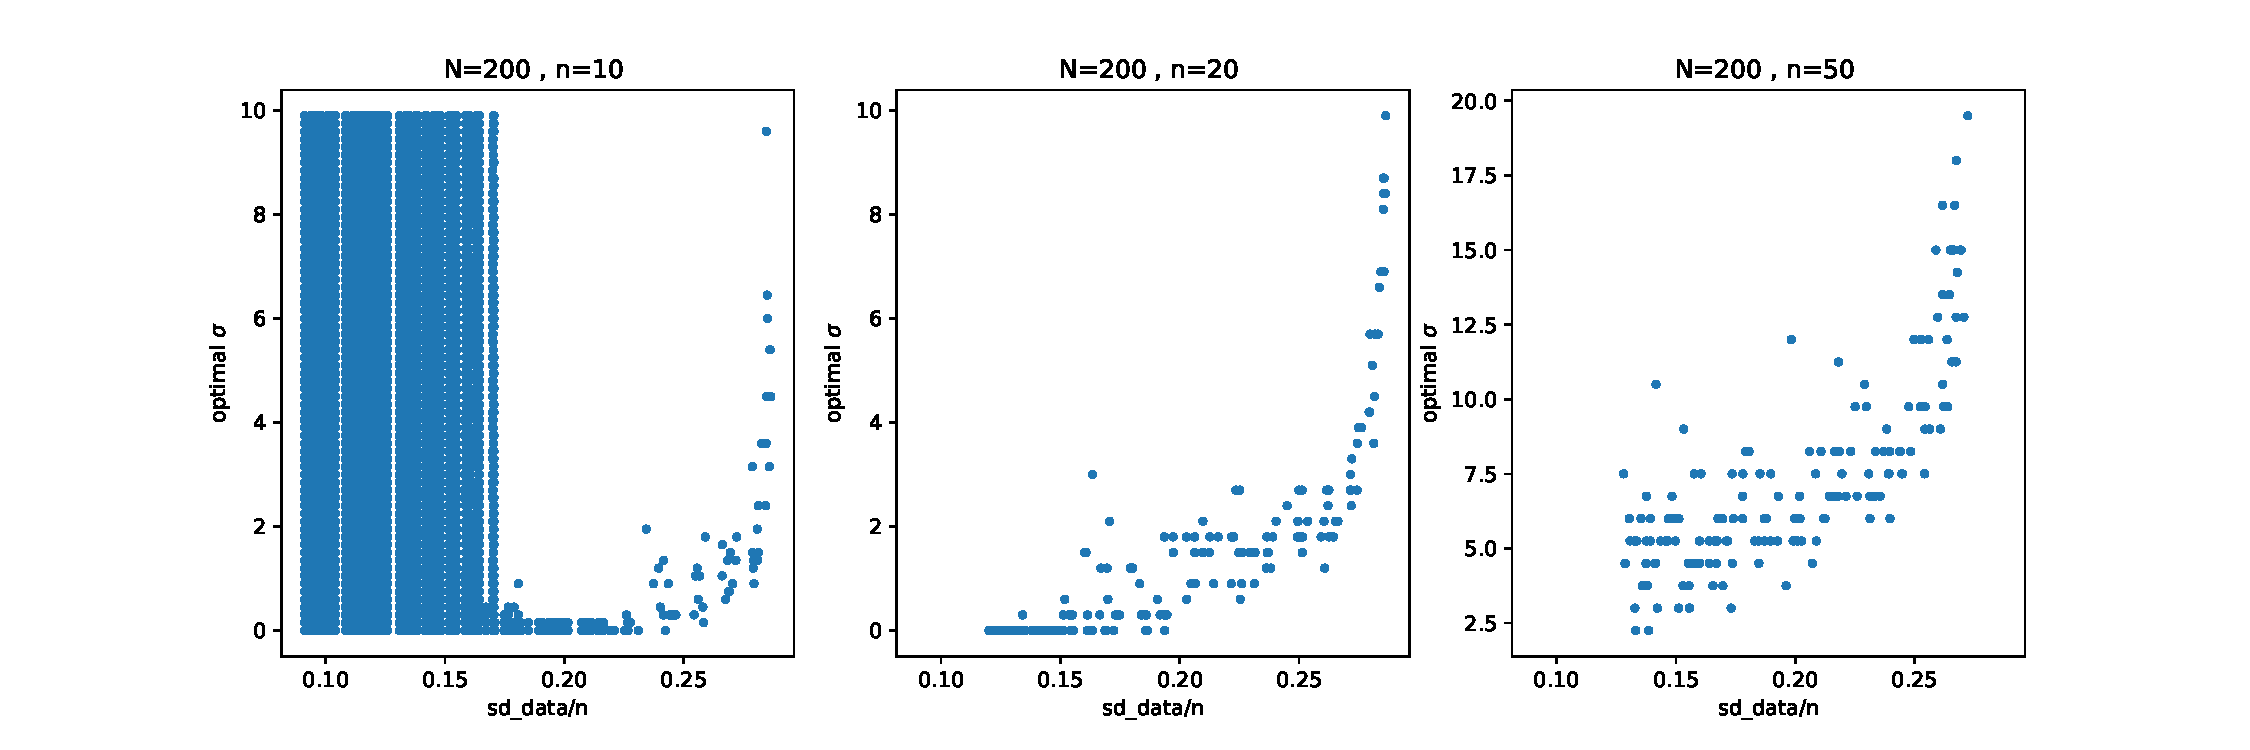
\includegraphics[width=\linewidth]{figures/2_4_sd_data_sameN200diffn.pdf}\label{fig_optimSigma_diff_n_sd_data}}
	\subfigure[]{
		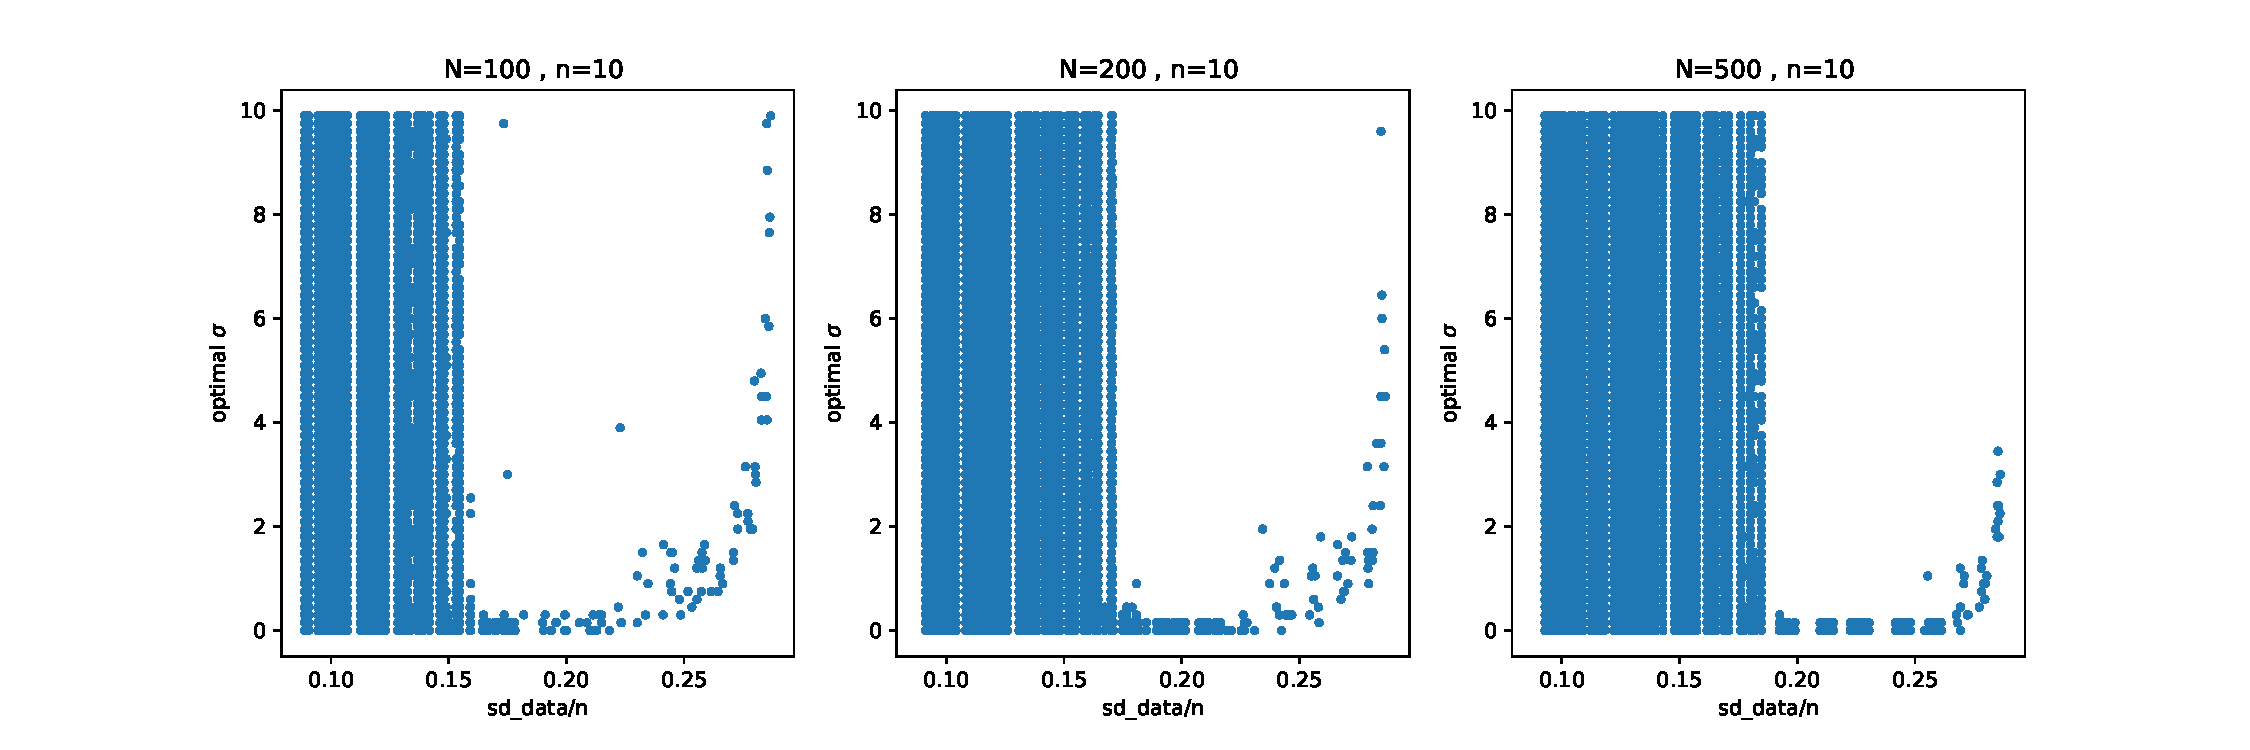
\includegraphics[width=\linewidth]{figures/2_4_sd_data_samen10diffN.pdf}\label{fig_optimSigma_diff_N_sd_data}}
	\caption{x-axis: $\alpha^0$, y-axis: optimal $\sigma$}
\end{figure}

\end{document}  